\documentclass[12pt]{article}  
% \linespread{1.1}
% \bibliographystyle{plain}
% 请在以下的方括号中填写队伍控制号
\usepackage[2623768]{easymcm}  % 载入 EasyMCM 模板文件


\problem{C}  % 请在此处填写题号
% \usepackage{mathptmx}  % 这是 Times 字体，中规中矩 
\usepackage{palatino}  % mathpazo 这palatino是 COMAP 官方杂志采用的更好看的 Palatino 字体，可替代以上的 mathptmx 宏包
\usepackage{pdfpages}
\usepackage{longtable}
\usepackage{tabu}
\usepackage{threeparttable}
\usepackage{listings}
\usepackage{paralist}
\usepackage{setspace}



\usepackage{graphicx} 
\graphicspath{{img/}}

 \let\itemize\compactitem
 \let\enditemize\endcompactitem
% \let\enumerate\compactenum
% \let\endenumerate\endcompactenum
% \let\description\compactdesc
% \let\enddescription\endcompactdesc
% \usepackage{biblatex} 
% \usepackage{cite}
% \usepackage{natbib}

\newcommand{\upcite}[1]{\textsuperscript{\textsuperscript{\cite{#1}}}}


\title{From Eliminations to Fan Votes: Inference and Fair Voting Design for Dancing with the Stars}  % 标题

% 如需要修改题头（默认为 MCM/ICM），请使用以下命令（此处修改为 MCM）
%\renewcommand{\contest}{MCM}
% 文档开始
\begin{document}
	\begin{abstract}
		
		As a global phenomenon in televised dance competitions, Dancing with the Stars (DWTS) commands a vast audience across dozens of countries, with its U.S. adaptation maintaining exceptional popularity throughout its 34 seasons. By integrating linear regression, a semi-supervised latent variable Bayesian framework, and Monte Carlo methods, we construct a comprehensive model to predict audience voting outcomes, providing both predicted values and confidence intervals. We further design a competition format that is both fairer and more engaging.
		
		\noindent \textbf{In task 1, we infer fan votes.}
		We replay all seasons under the \emph{Rank} and \emph{Percentage} rules using inferred weekly fan shares $\hat p_{i,s,t}$, and run counterfactual \emph{Bottom-2 + Judges’ Save} simulations. System-level effects are measured by season-level \textbf{disagreement/override rates} (primary metric) with uncertainty from \textbf{posterior-averaged estimates and credible intervals}. We find frequent large divergences ($\mathrm{DR}_s>0.6$), stronger fan overrides under Percentage, and late-season (Weeks 7--10) concentration of Bottom-2+Save reversals, especially under Percentage. Thus, \textbf{Percentage best preserves audience preference but should be paired with Bottom-2 + Judges’ Save to clip extreme fan-driven distortions while largely preserving strong-performer outcomes}.
		
		\noindent \textbf{In task 2, we compare voting rules and controversies.}
		We replay all seasons under the \emph{Rank} and \emph{Percentage} rules using inferred weekly fan shares $\hat p_{i,s,t}$, and run counterfactual \emph{Bottom-2 + Judges’ Save} simulations. We find frequent large divergences ($\mathrm{DR}_s>0.6$), stronger fan overrides under Percentage, and late-season (Weeks 7--10) concentration of Bottom-2+Save reversals, especially under Percentage. Thus, \textbf{Percentage best preserves audience preference but should be paired with Bottom-2 + Judges’ Save to clip extreme fan-driven distortions while largely preserving strong-performer outcomes}.
		
		\noindent \textbf{In task 3, we have a survival determinant Analysis.}
		To quantify the drivers of survival, we standardized the data via Probit transformation, and employed OLS regression as well as nonlinear interaction models to explore the impacts of celebrities' inherent attributes and partner effects on judges' scores and fan support, thereby analyzing the causes of discrepancies between the two parties. 
		
		\noindent \textbf{In task 4, 
			alternative elimination rules are designed and evaluated} to balance fairness and excitement under unobserved fan votes. Using \textbf{Monte Carlo season replays} driven by posterior fan-share draws, we compare format such as Entertainment-First Scheme (V1) and Fairness-Adjusted Blend (V2) with base model. As a result, V1 yields limited correction of popularity-driven runs, while V2 markedly reduces technical shocks without killing suspense, \textbf{motivating a V1-early/V2-late hybrid as the preferred policy}.
		
		\noindent Finally, based on our research findings, we provided the organizing committee with concrete, actionable recommendations: optimizing the casting matrix and restructuring voting weights.
		
		
		\medskip
		\noindent \textbf{Keywords}:\quad Bayesian Inference \quad Monte-Carlo Simulation 
		\quad Surprise Index \quad Retrospective Inference  \quad DWTS 
		
		
	\end{abstract}
	
	\maketitle  % 生成 Summary Sheet
	
	\tableofcontents
	


% 正文开始
% Chapter 1: Introduction
\section{Introduction}

\subsection{Problem Background}

\emph{Dancing with the Stars} (DWTS)   \textsuperscript{\cite{dwts_wiki}} combines two signals to determine weekly eliminations and final placements: judges’ numerical scores (technical merit) and audience votes (fan preference). Fan vote totals are not released, and the show has changed how the two signals are aggregated across seasons (rank, percentage/share, and later a Bottom-2 judges’ save), leading to recurring judge--fan discrepancies and controversy.

Given only judges’ scores, contestant attributes, and realized outcomes, we must infer weekly fan support consistent with observed eliminations, quantify uncertainty in those estimates, and use them to evaluate and propose voting systems (rank vs.\ percentage, with/without judge intervention) that are more ``fair'' or otherwise ``better'' (e.g., more exciting), supported by counterfactual season simulations.


\subsection{Problem Restatement}
We restate the problem into four core tasks addressed in this paper.

\begin{enumerate}
	\item \textbf{Inference of Fan Support: }
	Estimate latent weekly fan vote shares $p_{i,s,t}$ for each contestant and week, and evaluate
	whether these estimates are consistent with observed eliminations, including uncertainty.
	
	\item \textbf{Comparison of Voting Rules: }
	Using inferred $p_{i,s,t}$, we replay each season under \textit{rank} and \textit{percentage} aggregation to
	compare elimination paths and final placements; we then analyze controversial contestants as case studies and test an additional Bottom-2 judges' choice rule; based on the
	aggregate and case-level evidence, we recommend a voting method (and whether to include Bottom-2) for
	future seasons.
	
	
	\item \textbf{Explanation of Performance–Popularity Discrepancies: }
	Model how celebrity attributes (e.g., age, industry) and professional-partner effects relate to
	competition success, and test whether these factors impact judges' scores and fan votes differently.
	
	\item \textbf{Design of an Improved Elimination System:}
	Design an alternative weekly rule combining judges and fans that improves fairness and/or
	entertainment value, and justify it using evidence from simulations and empirical comparisons.
\end{enumerate}



\subsection{Our work}
\begin{enumerate}
	
	\item \textbf{Problem 1 (Inference of Fan Support): }
	We build a semi-supervised latent-variable model: a pooled mixed-effects popularity component
	produces a week-specific prior mean on fan support, eliminations are linked via a Softmin
	choice likelihood on the combined judge--fan signal, and a Dirichlet posterior update on the
	simplex is carried out via importance sampling to obtain posterior draws $p^{(b)}_{i,s,t}$; we
	then verify reliability by checking elimination-consistency and posterior-uncertainty behavior.
	
	
	
	\item \textbf{Problem 2 (Comparison of Voting Rules): }
	We replay each season under \textit{rank} and \textit{percentage} aggregation using $p^{(b)}_{i,s,t}$,
	quantify how elimination paths/placements change, and run case studies for controversial contestants
	(e.g., Rice/Cyrus/Palin/Bones) including a Bottom-2 judges' choice variant; we then recommend a rule
	(and whether to include Bottom-2) based on aggregate and case-level evidence.
	
	\item \textbf{Problem 3 (Explanation of Performance–Popularity Discrepancies): }
	We model competition outcomes with celebrity attributes (age, industry) and professional-partner
	effects, estimating separate pathways for judges versus fans and testing whether ``exceeding
	expectations'' predicts subsequent fan-support growth.
	
	\item \textbf{Problem 4 (Design of an Improved Elimination System): }
	We propose two improved weekly rules (excitement-oriented vs.\ fairness-oriented) and evaluate them
	through posterior-driven Monte-Carlo season replays, reporting large-sample impacts (by archetype)
	and controversy-case outcomes to support a producer-facing recommendation.
	
\end{enumerate}






% \section{Introduction}
% \subsection{Problem Background}
% Here is the problem background ...

% Two major problems are discussed in this paper, which are:
% \begin{itemize}
	%     \item Doing the first thing.
	%     \item Doing the second thing.
	% \end{itemize}

% \subsection{Literature Review}
% A literatrue\cite{1} say something about this problem ...

% \subsection{Our work}
% We do such things ...

% \begin{enumerate}[\bfseries 1.]
	%     \item We do ...
	%     \item We do ...
	%     \item We do ...
	% \end{enumerate}










% Chapter 2: 模型准备
\section{Preparation for Modeling}
\subsection{Model Assumptions}
\begin{enumerate}
	\setlength{\parsep}{0ex} %段落间距
	\setlength{\topsep}{2ex} %列表到上下文的垂直距离
	\setlength{\itemsep}{1ex} %条目间距
	
	\item \textbf{(Problem 1,2,4)}  Eliminations are modeled only on regular single-elimination weeks, and the weekly alive set $A_{s,t}$ is correctly identified.
	
	\item \textbf{(Problem 1,3)} Each week, we treat judges' scores as a \emph{relative performance ranking} among the remaining couples, and rescale this ranking (or scores) so it is comparable across weeks/seasons.
	
	\item \textbf{(Problem 1)} Each week’s fan voting is modeled as a vote-share vector $p_{s,t}$ (all entries positive and summing to 1), whose expected pattern $q_{s,t}$ is given by a softmax model.
	
	\item \textbf{(Problem 1)} Elimination is probabilistic rather than deterministic: couples with worse \emph{combined judge-and-fan signals} are more likely to be eliminated, with a temperature parameter governing the degree of randomness.
	
	
	\item \textbf{(Problem 1)} Actual weekly fan shares vary around the trend $q_{s,t}$; we model this variation with a Dirichlet distribution centered at $q_{s,t}$ and use posterior samples to quantify uncertainty in $p_{s,t}$.
	
	\item \textbf{(Problem 2,4)} Counterfactual evaluations assume invariance: changing the aggregation/elimination rule does not change the underlying judge scores or the underlying weekly fan preference distribution.
	
	\item \textbf{(Problem 3)} Within a season, the judging standard is stable enough that changes in the transformed judge signal track true performance improvement rather than rubric drift.
	
	\item \textbf{(Problem 3)} Fan support is comparable across seasons at matched checkpoints (e.g., Week 1 / mid-season / final), but not directly comparable across different weeks within the same season due to changing competition sets.
	
	\item \textbf{(Problem 2,4)} When a Bottom-2 judges' save is applied, judges eliminate the technically weaker couple among the bottom two according to the judge signal.
\end{enumerate}



\subsection{Notations}
\begin{table}[H]
	\centering
	\small
	\begin{tabular}{ll}
		\hline
		\hline
		\multicolumn{1}{c}{\textbf{Notations}} & \textbf{Definition}\\
		\hline
		$s$ & season index \\
		$t$ & week index within season \\
		$i$ & contestant (celebrity) index \\
		$A_{s,t}$ & alive set in week $(s,t)$ \\
		$J_{i,s,t}$ & judges' signal for $i$ in week $(s,t)$ (normalized) \\
		$p_{i,s,t}$ & latent fan vote share for $i$ in week $(s,t)$ \\
		$q_{i,s,t}$ & prior mean of $p_{i,s,t}$ (trend prediction) \\
		$\kappa$ & Dirichlet concentration (fan-volatility control) \\
		$S_{i,s,t}$ & combined score used for elimination \\
		$\tau$ & softmin temperature in elimination likelihood \\
		$i^*(s,t)$ & observed eliminated contestant in week $(s,t)$ \\
		$\mathrm{PCP}_{s,t}$ & posterior prob. of matching $i^*(s,t)$ \\
		$\widehat e^{rank}_{s,t}$ & predicted eliminatee under rank scheme \\
		$\widehat e^{pct}_{s,t}$ & predicted eliminatee under percentage scheme \\
		$\text{Bottom2}(s,t)$ & two lowest-$S$ contestants in week $(s,t)$ \\
		\hline
		\hline
	\end{tabular}
	\caption{Notations Table (Core Symbols)}
\end{table}




\subsection{Data Preprocessing}

\begin{enumerate}
	\setlength{\parsep}{0ex} %段落间距
	\setlength{\topsep}{2ex} %列表到上下文的垂直距离
	\setlength{\itemsep}{1ex} %条目间距
	
	\item \textbf{Structural zero handling:} Judge scores recorded as zeros after a contestant’s elimination were recoded as missing values (NaN), while original N/A entries were preserved, to avoid systematic bias in weekly aggregates, rankings, and percentage-based measures.
	
	\item \textbf{Outcome parsing and withdrawal exclusion:} Textual season outcomes were standardized into structured fields (\texttt{elim\_week\_result}, \texttt{is\_withdrew}, \texttt{is\_place}), and mid-season withdrawals were excluded so that eliminations reflect the intended competition mechanism.
	
	\item \textbf{Season length and activity window definition:} For each season, the true competition length was identified and each contestant’s activity horizon (\texttt{active\_until}) was constructed, yielding a well-defined weekly alive set \(A_{s,t}\) for all subsequent analyses.
	
	\item \textbf{Construction of analysis-ready tables:} Starting from the cleaned wide roster table, we reshaped judge scores into a judge-level long table, aggregated them into a weekly panel with \texttt{total/mean\_judge\_score} and \texttt{n\_judges\_scored}, derived rule-specific inputs (\texttt{judge\_rank}, \texttt{judge\_percent}), and created auxiliary roster and elimination-event tables to explicitly encode the sample space and week-end outcomes.
	
	\item \textbf{Cross-season pooling via rank normalization (used only in Problem~3):} 
	To enable cross-season comparability, weekly judge ranks \(R^J_{i,t}\) within the eligible set were mapped to standardized normal scores using
\begin{equation} 
	Z^J_{i,t}=\Phi^{-1}\!\left(\mathrm{clip}\!\left(1-\frac{R^J_{i,t}-0.5}{N_{s,t}},\,0.001,\,0.999\right)\right),
\end{equation}
	and fan support was summarized by extracting probability snapshots at W1, W6, and the final week, producing a pooled contestant--season table for downstream modeling in Problem~3 only.
	
\end{enumerate}















\section{Problem 1: Latent Fan Support Reconstruction}

Since true fan vote totals are unobserved, we adopt a semi-supervised strategy: we learn a latent fan-support structure that maximizes the likelihood of observing the historical elimination sequence, and then use Bayesian inversion to estimate weekly fan shares.

\subsection{Model Framework}


\paragraph{Data Standardization:}

Let $A_{s,t}$ denote the \textbf{alive set} (contestants active in season $s \in \{1,\dots,S\}$ and week $t \in \{1,\dots,T_s\}$). For each contestant $i \in A_{s,t}$, we standardize the raw judge scores into a unified probability metric $J_{i,s,t} \in [0,1]$ to enable cross-era modeling:

\begin{itemize}
	\item \textbf{Percentage Era:} We normalize the raw score $T_{i,s,t}$ against the weekly sum:
	\begin{equation}
		J_{i,s,t} = \frac{T_{i,s,t}}{\sum_{k \in A_{s,t}} T_{k,s,t}}
	\end{equation}
	\item \textbf{Rank Era:} We convert the within-judge rank sum $R_{i,s,t}$ (where lower is better) into a share using a Softmax transformation to ensure magnitude comparability:
	\begin{equation}
		J_{i,s,t} = \frac{\exp(-R_{i,s,t})}{\sum_{k \in A_{s,t}} \exp(-R_{k,s,t})}
	\end{equation}
\end{itemize}




\paragraph{Latent Variable Formulation:}

We define the unnormalized ``popularity potential'' $\eta_{i,s,t}$ using a mixed-effects linear model.
To keep the model parsimonious and identifiable from elimination outcomes, we restrict the covariates to
the most stable, high-signal variables and avoid weakly-informative high-cardinality encodings (e.g.,
industry/country one-hot), which did not yield consistent predictive gains.

\begin{equation} \label{eq:latent_score}
	\eta_{i,s,t} = 
	\underbrace{\mathbf{x}_{i,s,t}^{\top}\boldsymbol{\beta}}_{\text{Observed Signal (Judge \& Age)}} 
	+ \underbrace{u_{i,s}}_{\text{Static Star Power}}, 
	\quad u_{i,s} \sim \mathcal{N}(0, \sigma_u^2)
\end{equation}
Here, $\mathbf{x}_{i,s,t}$ contains only (i) the contestant's \emph{current-week} judge performance metric
(e.g., $J_{i,s,t}$ defined within the alive set) and (ii) the contestant age in that season
(e.g., $\text{Age}_{i,s}$, centered and scaled).
The coefficient vector $\boldsymbol{\beta}$ is pooled across all seasons, while the random intercept
$u_{i,s}$  \textsuperscript{\cite{laird1982}}captures persistent, contestant-specific fanbase strength that is not explained by dance quality.
\textbf{In short,} $\boldsymbol{\beta}$ is learned by maximum likelihood: after observing eliminations across
weeks, we choose the value of $\boldsymbol{\beta}$ that makes the observed elimination outcomes most probable
under our elimination likelihood (ignoring any regularization term).


The \textbf{Expected Fan Share} $q_{i,s,t}$ is obtained by mapping $\eta$ to the simplex within the alive set:
\begin{equation} \label{eq:prior_mean}
	q_{i,s,t} = \frac{\exp(\eta_{i,s,t})}{\sum_{k \in A_{s,t}} \exp(\eta_{k,s,t})}
\end{equation}

\paragraph{Likelihood Maximization:}

To connect latent support to binary outcomes, we define the Combined Score $C_{i,s,t} = J_{i,s,t} + q_{i,s,t}$. We model the probability that contestant $i^*$ is eliminated using a \textbf{Softmin Choice Rule} with temperature $\tau$:
\begin{equation}
	\Pr(i^* \text{ elim} \mid A_{s,t}) = \frac{\exp(-C_{i^*,s,t}/\tau)}{\sum_{k \in A_{s,t}} \exp(-C_{k,s,t}/\tau)}
\end{equation}

Model parameters $\Theta = \{b, \beta, u, \tau\}$ are estimated by minimizing the penalized negative log-likelihood over all training weeks $\mathcal{T}$:
\begin{equation}
	\mathcal{L}(\Theta) = \sum_{(s,t) \in \mathcal{T}} \left[ \frac{C_{i^*,s,t}}{\tau} + \log \sum_{k \in A_{s,t}} \exp\left(-\frac{C_{k,s,t}}{\tau}\right) \right] + \lambda_{\beta}\|\beta\|_2^2 + \lambda_u\|u\|_2^2
\end{equation}
The $\ell_2$ regularization terms ($\lambda$) prevent overfitting to specific seasons, ensuring $\beta$ captures generalizable rules.\textsuperscript{\cite{hoerl1970}}

\paragraph{Bayesian Posterior Update:}

The trend $q_{i,s,t}$ represents the "average" trajectory. To capture weekly volatility (e.g., viral moments or scandals), we treat the "realized" fan vote $p_{s,t}$ as a random variable and update it given the observed elimination $i^*$.
We employ a Dirichlet-Softmin Bayesian filter\textsuperscript{\cite{gelman2013}}:
\begin{enumerate}
	\item \textbf{Dirichlet Trend Regularization:}
	$p_{s,t} \sim \mathrm{Dirichlet}(\alpha_{s,t}=\kappa\,q_{s,t})$, where $\kappa$ controls adherence to the historical fan-support trend.\textsuperscript{\cite{bishop2006}}
	\item \textbf{Elimination Consistency Constraint:}
	The observed eliminatee $i^*$ induces a likelihood that favors vote vectors $p_{s,t}$ under which $i^*$ has high elimination probability.
\end{enumerate}

The posterior distribution is derived via Bayes' Theorem:
\begin{equation} \label{eq:posterior_update}
	\pi(p_{s,t} \mid i^*_{\text{elim}}) \propto \underbrace{\left( \prod_{i \in A_{s,t}} p_{i,s,t}^{\kappa q_{i,s,t} - 1} \right)}_{\text{Prior Belief}} \cdot \underbrace{\left( \frac{\exp(-(J_{i^*,s,t} + p_{i^*,s,t})/\tau)}{\sum_{k} \exp(-(J_{k,s,t} + p_{k,s,t})/\tau)} \right)}_{\text{Evidence Correction}}
\end{equation}
Since this is analytically intractable, we estimate $p_{s,t}$ via Importance Sampling.


\paragraph{Visual Interpretation:}
Figure \ref{fig:week_trajectory} visualizes the \textbf{posterior} fan support trajectories (post-update). The \textbf{vertical stratification} is determined by the prior $u_{i,s}$ (Static Star Power), while the \textbf{weekly fluctuations} reveal the posterior corrections driven by Eq. \eqref{eq:posterior_update}: notice how the trajectories dynamically dip to account for unexpected eliminations, ensuring consistency with reality.



\begin{figure}[htbp]
	\centering
	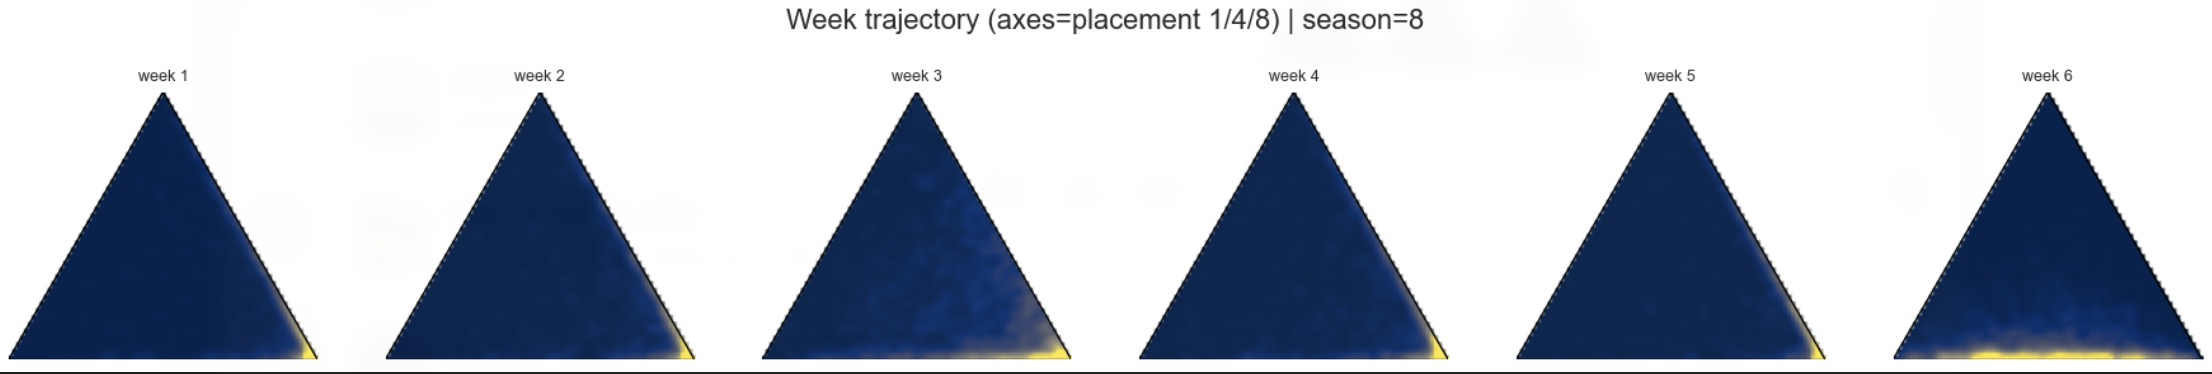
\includegraphics[width=0.9\linewidth]{week_trajectory.jpg}
	\caption{\textbf{Inferred Fan Support Trajectories (Season 8).} Each triangle is a posterior heatmap of the weekly fan-share simplex (axes = placement 1/4/8): left corner = eventual \#1, right corner = eventual \#4, top corner = eventual \#8. Yellow indicates where posterior mass concentrates after conditioning on that week's elimination history; the mass drifting from the lower-right toward the bottom edge reflects a posterior update that moves away from \#8 (elimination risk) and shifts the implied outcome from \#4-like to \#1-like support.}
	\label{fig:week_trajectory}
\end{figure}




\subsection{Model Evaluation}

To rigorously validate our latent variable framework, we employ a tri-layered evaluation strategy: (1) \textbf{Internal validity} (Internal Consistency), (2) \textbf{External validity} (External Realism), and (3) \textbf{Uncertainty} (Risk Quantification).

\subsubsection{Internal validity}

\noindent
\textbf{Does the inferred fan vote reproduce weekly eliminations?}
We answer this in two complementary ways: (i) exact week-by-week reconstruction, and (ii) graded, season-level consistency that distinguishes near-misses from catastrophic failures.

\medskip
\noindent
\textbf{(1) Top-1 accuracy:}
We compare our inference-driven \texttt{torch\_model} to an \textbf{XGBoost} baseline (same features) under the strict Top-1 metric:
\begin{equation}
	\mathcal{A} = \frac{1}{N} \sum_{s,t} \mathbf{1}\left\{ \arg\min_{i \in A_{s,t}} \hat C_{i,s,t} = i^*(s,t) \right\},
\end{equation}
where $A_{s,t}$ is the alive set, $\hat C_{i,s,t}$ is the model-implied risk/combined score, and $i^*(s,t)$ is the observed eliminatee.
The baseline achieves $\mathcal{A}=0.806554$, while \texttt{torch\_model} reaches $\mathcal{A}=0.952092$, and wins in \emph{every} season (Fig.~\ref{fig:acc_season}), indicating that the inferred fan votes are highly consistent with observed eliminations.

\begin{figure}[htbp]
	\centering
	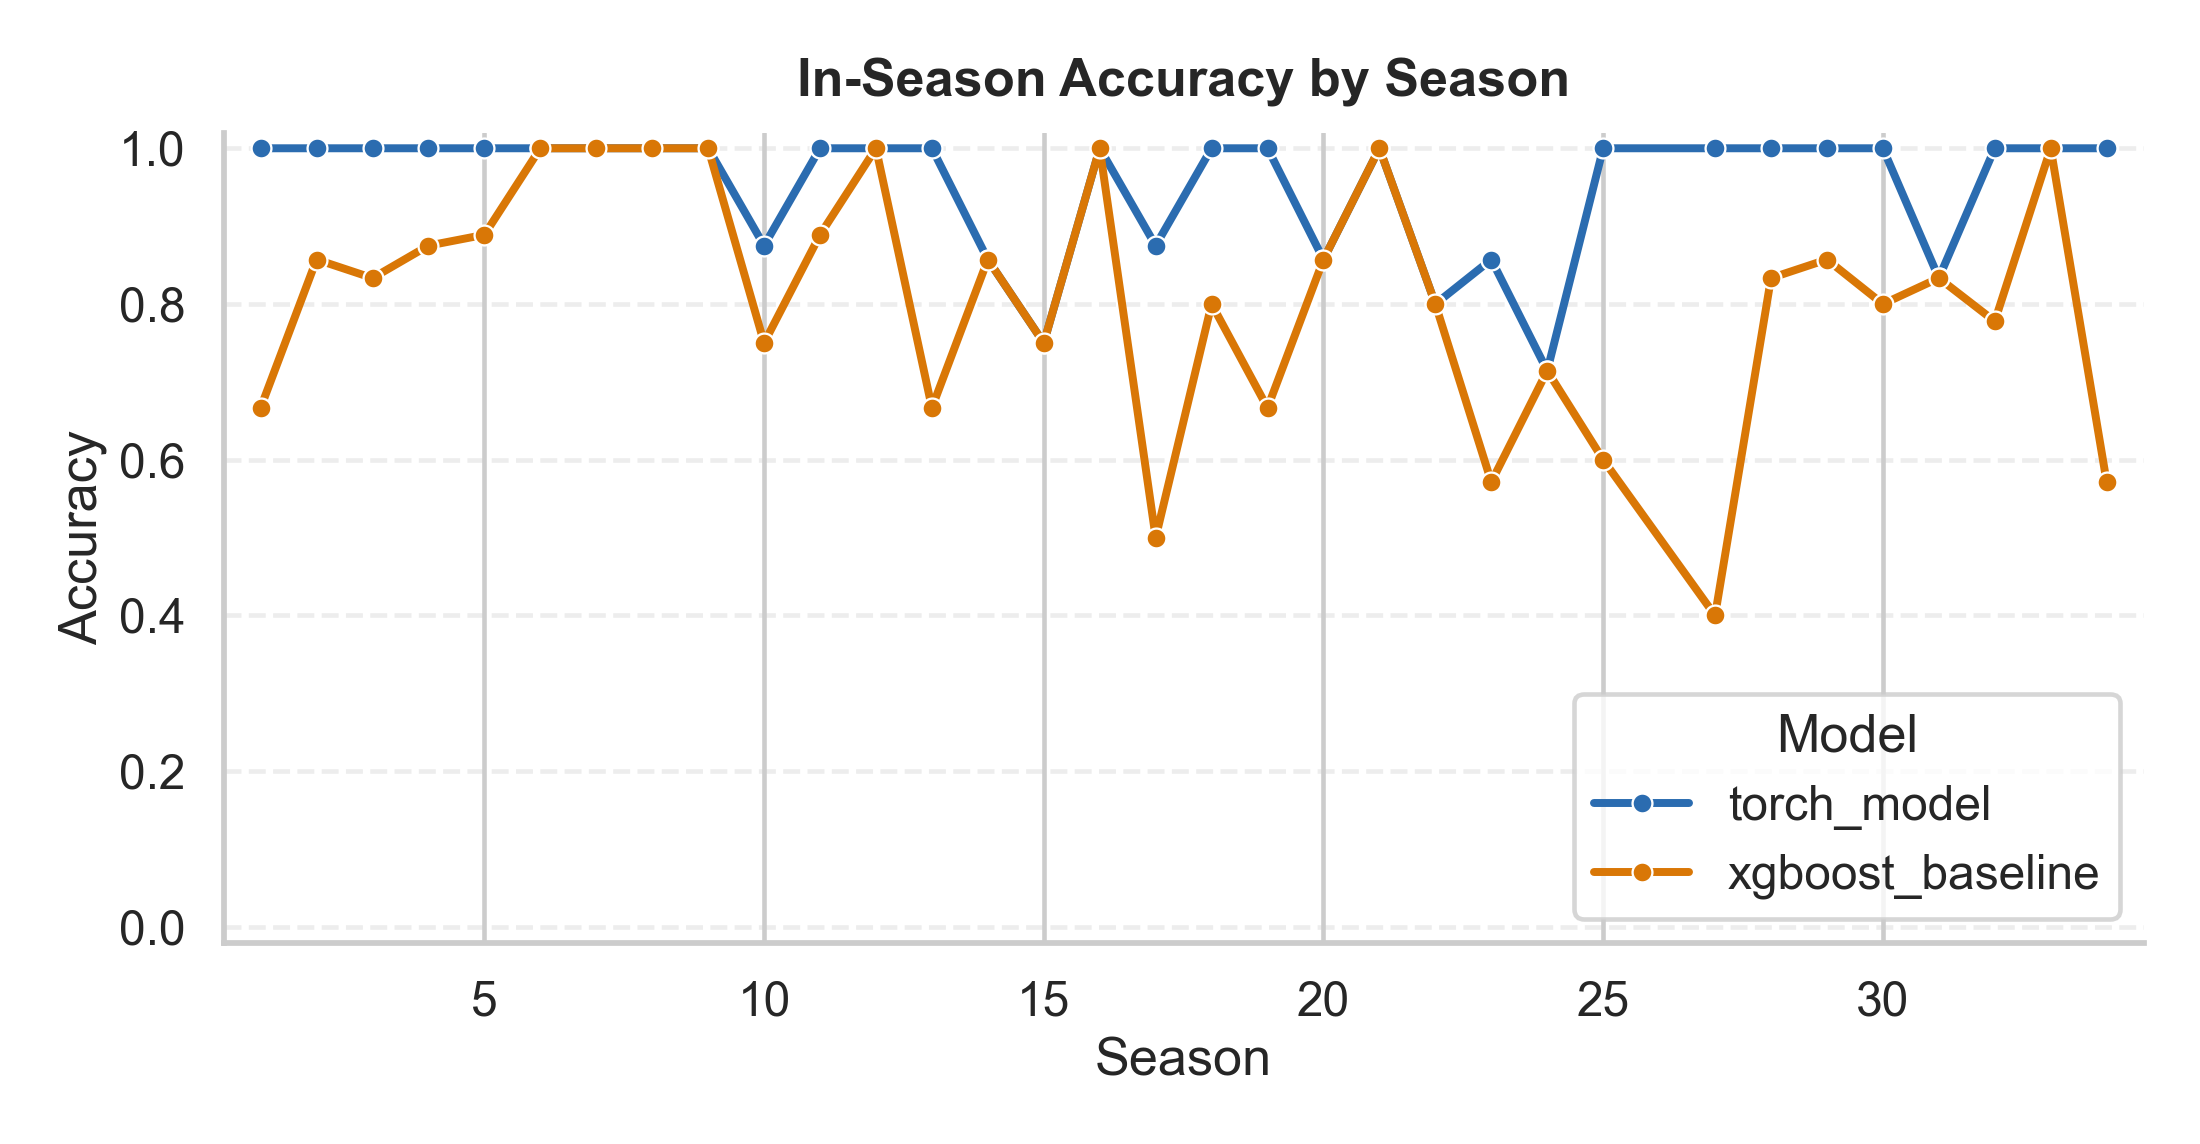
\includegraphics[width=0.6\linewidth]{1_model_accuracy_line.png}
	\caption{\textbf{In-Season Accuracy by Season.} The proposed \texttt{torch\_model} consistently outperforms the \texttt{xgboost\_baseline} in Top-1 elimination reconstruction accuracy.}
	\label{fig:acc_season}
\end{figure}

\medskip
\noindent
\textbf{(2) Graded consistency beyond Top-1:}
Top-1 accuracy assigns the same penalty to a near-miss (true eliminatee ranked 2nd/3rd most-at-risk) and a catastrophic miss (ranked very safe). We therefore evaluate whether the model recovers the \emph{set} of contestants who should have exited by each stage of the season.

For season $s$, let $E_{s,k}$ be the set of contestants actually eliminated by the end of the $k$-th elimination event, and let $\widehat{E}_{s,k}$ be the set produced by a deterministic replay under the model (each event removes the lowest-$m$ contestants by $\hat C$, matching the observed number of eliminations).
Define $n_{s,k}=|E_{s,k}|$ and $n'_{s,k}=|E_{s,k}\cap \widehat{E}_{s,k}|$, and score
\begin{equation}
	\label{eq:cum_consistency}
	\mathcal{S}_s
	=
	\frac{1}{H_{K_s}}
	\sum_{k=1}^{K_s}
	\frac{1}{k}\cdot \frac{n'_{s,k}}{n_{s,k}},
	\qquad
	H_{K_s}=\sum_{k=1}^{K_s}\frac{1}{k}.
\end{equation}
Averaged across seasons, we obtain $\bar{\mathcal{S}}=0.78$, showing substantial order-level agreement beyond exact-week hits.

\emph{Why can $\bar{\mathcal{S}}$ be lower than $\mathcal{A}$?}
This is not a contradiction: $\mathcal{A}$ is a one-step, week-local test (identify the single most at-risk contestant \emph{given the current alive set}), whereas $\mathcal{S}_s$ evaluates a multi-step \emph{trajectory}---small ranking errors early can propagate through the replay and keep the cumulative eliminated set mis-aligned for many subsequent stages.
In short, the model is very strong at predicting the next elimination, but reconstructing the entire season path from the start without additional information is intrinsically harder.




\subsubsection{External validity}

To verify the model's robustness under uncertainty, we first define a probabilistic consistency metric:


\noindent \textbf{Posterior Consistency Probability (PCP):}
An uncertainty-aware metric defined as the posterior probability that the model reproduces the observed elimination, estimated via Monte Carlo integration by the fraction of posterior fan-vote draws that correctly identify the eliminatee:
	\begin{equation}
		\text{PCP}_{s,t} = \frac{1}{B} \sum_{b=1}^B \mathbf{1}\left\{ \arg\min_{i} (J_{i,s,t} + p^{(b)}_{i,s,t}) = i^*(s,t) \right\}
	\end{equation}
	Here, the weight is uniform ($1/B$) for each sample $b$.


We validate the physical realism of the model against two structural hypotheses using these metrics.

\noindent\textbf{Hypothesis A: The Crowded Field Dilution:}
Intuitively, predicting the loser is harder when the candidate pool $|A_{s,t}|$ is large. Figure \ref{fig:pcp_alive} confirms this: PCP is lower in early weeks (high $|A_{s,t}|$) and converges to $\approx 1.0$ as the field narrows. This proves the model captures the \textbf{crystallization of fan bases}.

\noindent\textbf{Hypothesis B: The Popularity Premium:}
Does inferred $p_{i,s,t}$ reflect real popularity? We define the \textbf{Ranking Gap} $\Delta R_{i}$ as the discrepancy between a contestant's final placement and their average judge rank:
\begin{equation}
	\Delta R_{i} = \text{Rank}_{\text{Final}} - \text{Rank}_{\text{Judge}}
\end{equation}
Figure \ref{fig:ranking_gap} shows a strong positive correlation ($R^2 > 0.6$) between $\Delta R_i$ and our inferred Fan Rank. This confirms the model correctly identifies high latent support for contestants who "over-performed" their technical skill.

\begin{figure}[htbp]
	\centering
	\begin{minipage}[t]{0.48\linewidth}
		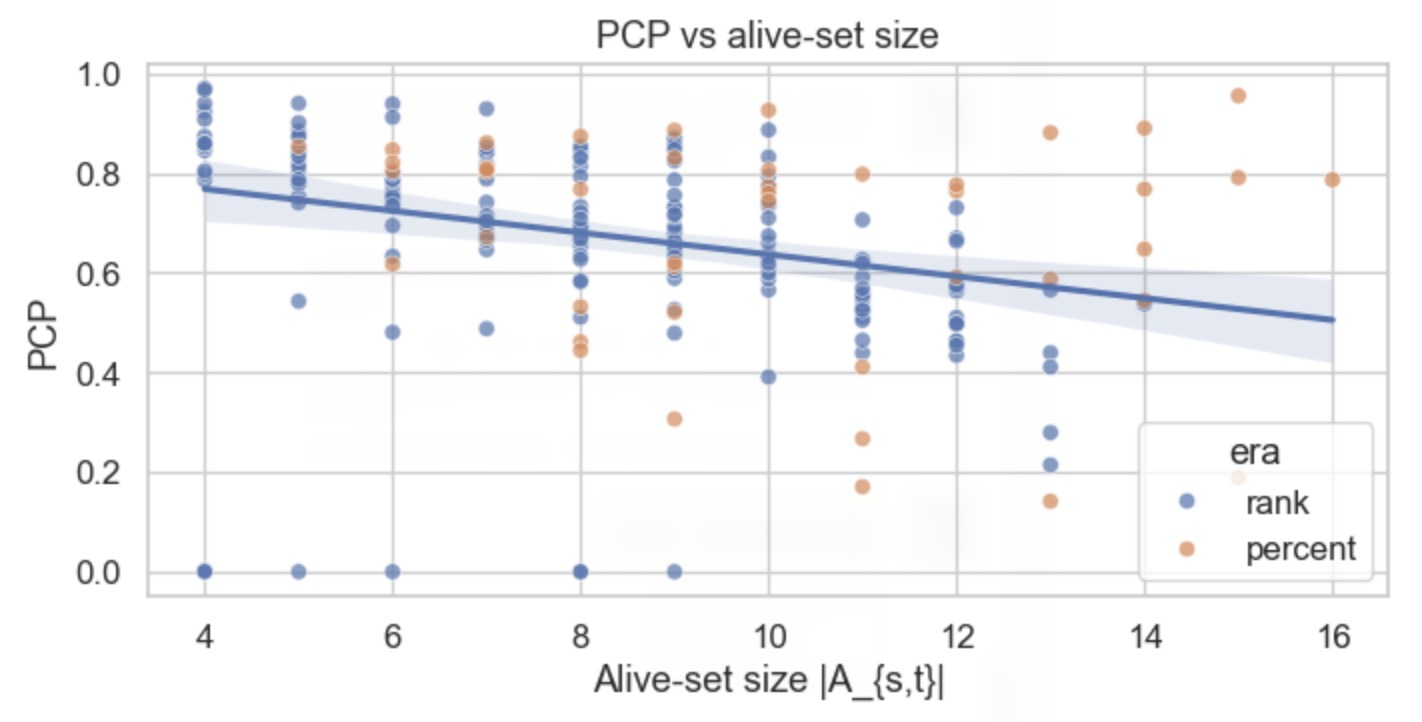
\includegraphics[width=\linewidth]{pcp_vs_alive.jpg}
		\caption{\textbf{Crowded Field Effect.} Consistency naturally increases as the alive set shrinks (from right to left).}
		\label{fig:pcp_alive}
	\end{minipage}
	\hfill
	\begin{minipage}[t]{0.48\linewidth}
		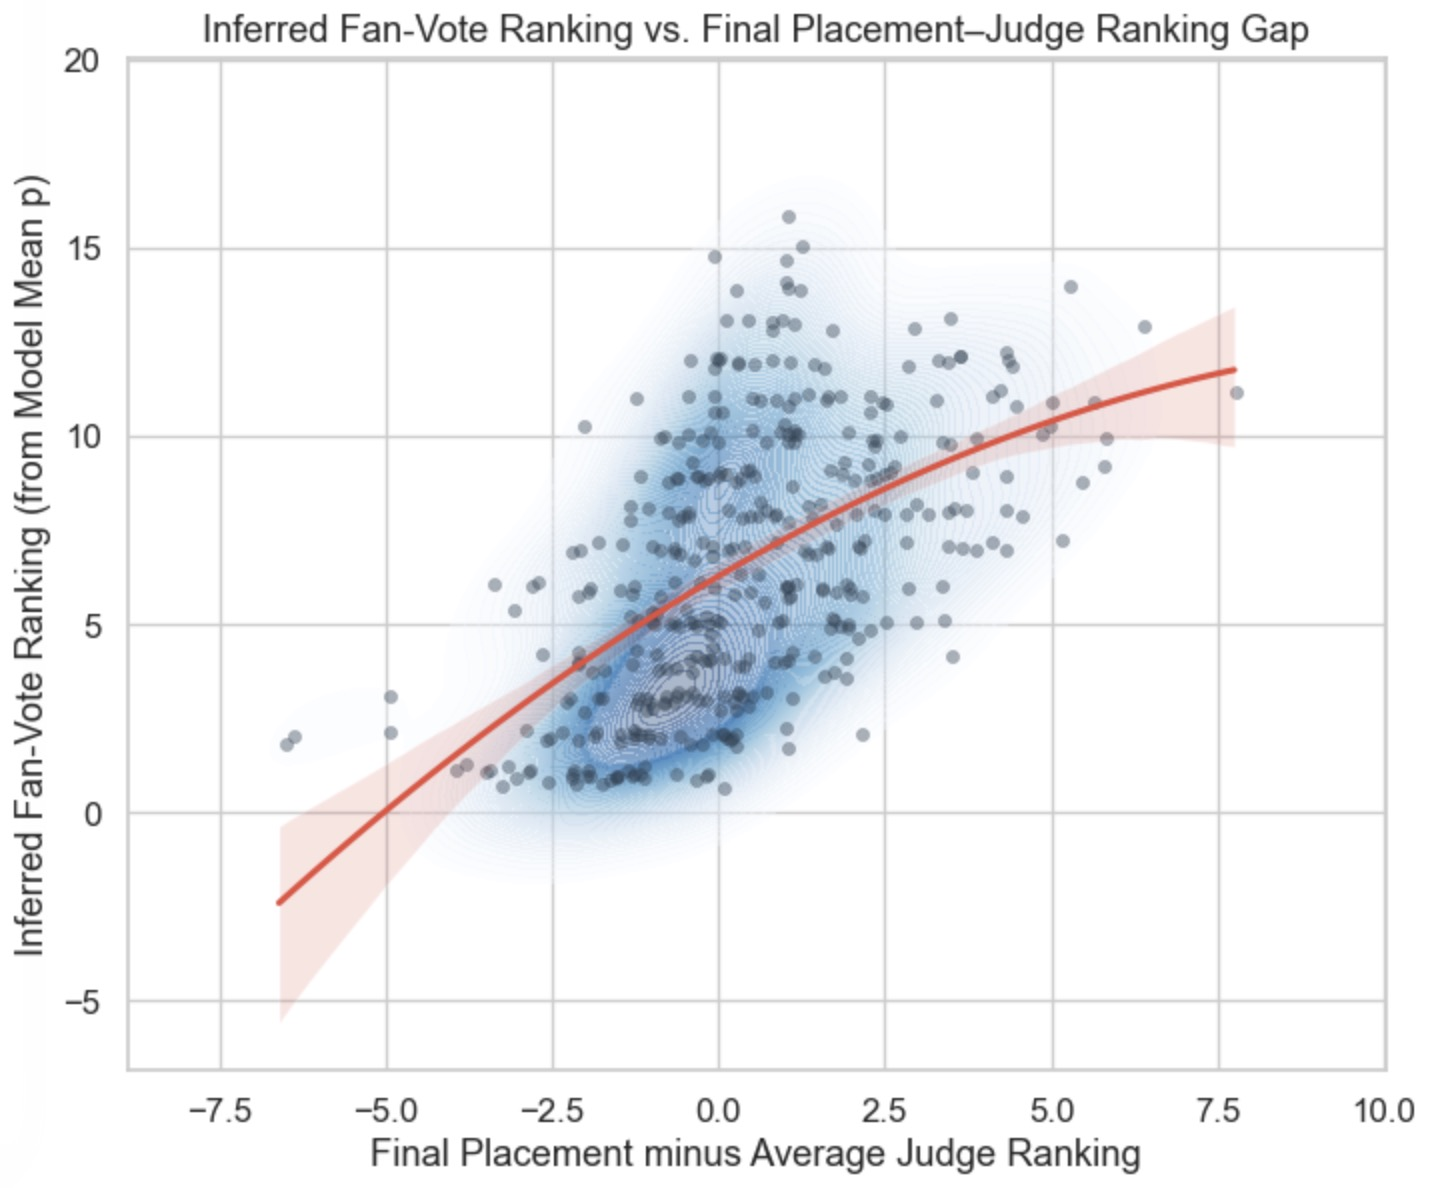
\includegraphics[width=\linewidth]{ranking_gap.jpg}
		\caption{\textbf{The Popularity Premium.} Inferred votes correlate with contestants who outperformed judge scores.}
		\label{fig:ranking_gap}
	\end{minipage}
\end{figure}


\subsubsection{Uncertainty}

Our key estimate is the latent weekly fan-vote \emph{share} vector
$p_{s,t}=(p_{i,s,t})_{i\in A_{s,t}}$ on the simplex.
Conditioning on the observed elimination, we obtain weighted posterior draws
$\{p^{(b)}_{i,s,t}\}_{b=1}^{B}$ (via a Dirichlet-centered prior and an elimination likelihood, approximated by importance sampling).
For each contestant-week, we report the posterior mean $\hat p_{i,s,t}$ and a \textbf{90\% credible interval}
\begin{equation}
\mathrm{CI}^{90}_{i,s,t}=\Big[Q^{w}_{0.05}(p_{i,s,t}),\;Q^{w}_{0.95}(p_{i,s,t})\Big],
\end{equation}
and summarize its tightness by the \textbf{relative interval width}
\begin{equation}
\mathrm{RW}_{i,s,t}=\frac{\mathrm{CI}^{90}_{i,s,t,\mathrm{high}}-\mathrm{CI}^{90}_{i,s,t,\mathrm{low}}}{\hat p_{i,s,t}+\epsilon}.
\end{equation}
Smaller $\mathrm{RW}_{i,s,t}$ means higher certainty in the inferred fan-vote share.

\textbf{Is certainty the same for every contestant/week? No.}
Figure~\ref{fig:rw_heatmap_s21} visualizes $\mathrm{RW}_{i,s,t}$ as a contestant--week heatmap for a representative season (Season 21).
Two patterns are clear: (i) uncertainty is \emph{heterogeneous across contestants within the same week} (rows differ sharply), and
(ii) uncertainty typically \emph{changes over the season} (columns vary), with several early-week contestants showing wide relative intervals
(bright cells) while late-stage survivors often exhibit tighter intervals (darker cells).
Blank cells indicate weeks after a contestant has been eliminated (not in $A_{s,t}$).
Therefore, our fan-vote totals come with \emph{contestant-week specific} uncertainty, rather than a single global confidence level.

\textbf{Diagnostic note: }
Since credible intervals are computed from weighted draws, we also track the effective sample size (ESS) per week and flag low-ESS weeks as less reliable, increasing $B$ to stabilize the reported intervals.

\begin{figure}[htbp]
	\centering
	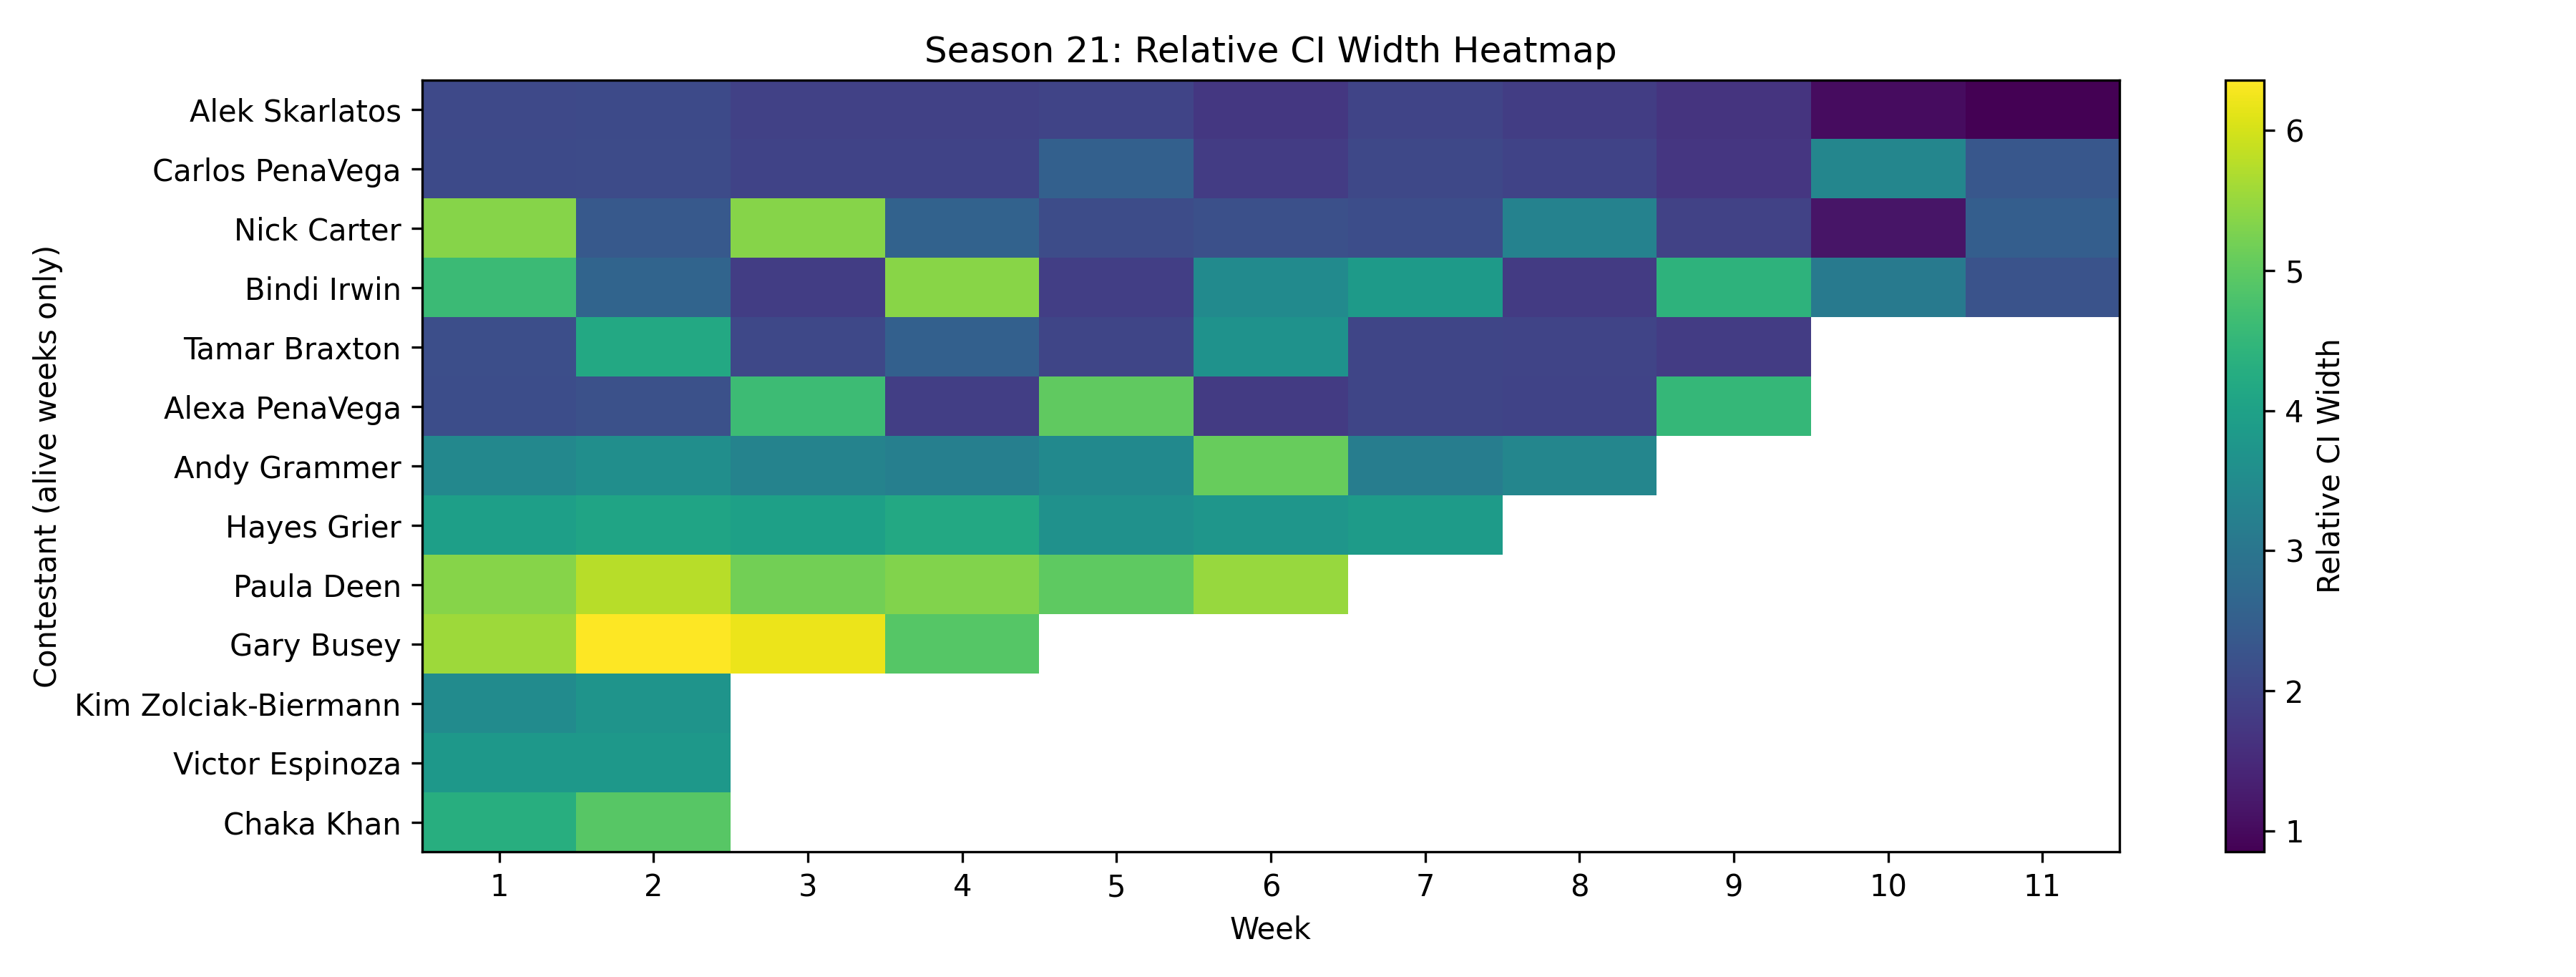
\includegraphics[width=0.95\linewidth]{1_fig2_ci_heatmap_S21.png}
	\caption{\textbf{Season 21: relative 90\% CI width of inferred fan-vote shares.}
		Each cell shows $\mathrm{RW}_{i,s,t}$ for contestant $i$ at week $t$ while alive; smaller values (darker) indicate higher certainty.
		Blank cells correspond to weeks after elimination.
		The heatmap shows that uncertainty is not constant: it varies across contestants and evolves over weeks.}
	\label{fig:rw_heatmap_s21}
\end{figure}




















\section{Problem 2: Rank vs.\ Percentage and the Bottom-2 Judges' Save}


We compare \textbf{Rank} vs.\ \textbf{Percentage} by replaying each season under both rules, then analyze \textbf{controversial contestants} with large judge--fan disagreement to see whether the rule choice would change their outcomes, and finally evaluate the added \textbf{Bottom-2 + Judges' Save} mechanism to quantify how much it corrects fan-driven eliminations.



\subsection{Systemic Divergence Metrics}

\paragraph{Rule Definitions:}
We consider two commonly used elimination rules that aggregate judges’ scores and fan support in fundamentally different ways.
Under the \emph{rank-based (ordinal)} rule, the contestant with the largest sum of judge rank and fan-vote rank is eliminated:
\begin{equation}
	\hat e^{\mathrm{rank}}_{s,t}=\arg\max_{i\in A_{s,t}}
	\Big(\mathrm{rank}(-T_{i,s,t})+\mathrm{rank}(-\hat p_{i,s,t})\Big).
\end{equation}
In contrast, the \emph{percentage-based (cardinal)} rule eliminates the contestant with the smallest combined share of normalized judge score and fan votes:
\begin{equation}
	\hat e^{\mathrm{pct}}_{s,t}=\arg\min_{i\in A_{s,t}}
	\left(\frac{T_{i,s,t}}{\sum_{k\in A_{s,t}}T_{k,s,t}}+\hat p_{i,s,t}\right).
\end{equation}

\paragraph{Disagreement Rate:}
To quantify how often these two rules lead to different elimination outcomes within a season, we define the disagreement rate
\begin{equation}
	DR_s=\frac{1}{|\mathcal{W}_s|}\sum_{t\in\mathcal{W}_s}\mathbb{1}\{\hat e^{\mathrm{rank}}_{s,t}\neq \hat e^{\mathrm{pct}}_{s,t}\}.
\end{equation}
Figure~\ref{fig:systemic_disagreement} reveals a bimodal pattern in $DR_s$, with frequent disagreement ($DR_s>0.6$) concentrated in late-season weeks when the alive set is small and judge scores are tightly clustered.

\begin{figure}[ht]
	\centering
	\begin{minipage}{0.48\textwidth}
		\centering 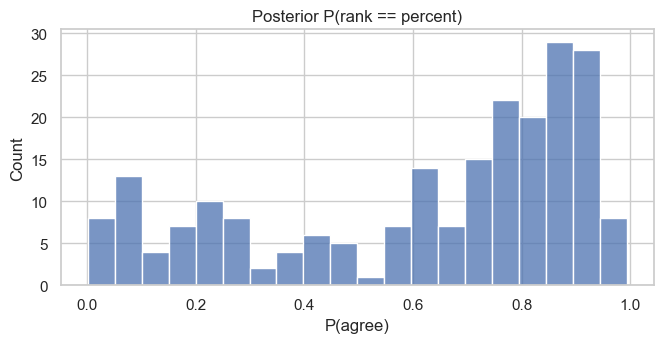
\includegraphics[width=\linewidth]{2_posterior_probability.png} \textbf{(a) Posterior Agreement}
	\end{minipage}
	\hfill
	\begin{minipage}{0.48\textwidth}
		\centering 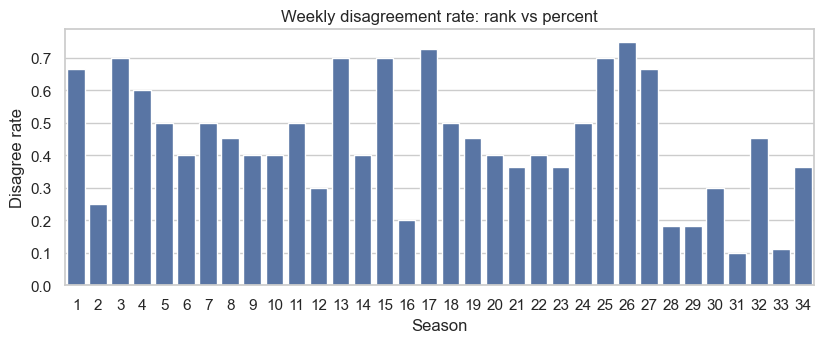
\includegraphics[width=\linewidth]{2_weekly_disagreement.png} \textbf{(b) Weekly Disagreement}
	\end{minipage}
	\caption{\textbf{Systemic Divergence.} Agreement is bimodal; disagreement spikes in specific seasons.}
	\label{fig:systemic_disagreement}
\end{figure}

\paragraph{Fan Bias:}
To quantify the extent to which fan votes overturn judges’ rankings, we define two season-level indicators for each method $m\in\{\mathrm{rank},\mathrm{pct}\}$.
The \emph{Override rate} measures how often the eliminated contestant differs from the judge-only loser,
\begin{align}
	\mathrm{Override}^{(m)}_s
	&=\frac{1}{|\mathcal{W}_s|}\sum_{t\in\mathcal{W}_s}\mathbb{1}\!\left\{\hat e^{(m)}_{s,t}\neq \arg\min_{k\in A_{s,t}} T_{k,s,t}\right\},
\end{align}
while \emph{Fan-worst elimination} captures the frequency with which the least-supported contestant by fans is eliminated,
\begin{align}
	\mathrm{FanWorstElim}^{(m)}_s
	&=\frac{1}{|\mathcal{W}_s|}\sum_{t\in\mathcal{W}_s}\mathbb{1}\!\left\{\hat e^{(m)}_{s,t}= \arg\min_{k\in A_{s,t}} \hat p_{k,s,t}\right\}.
\end{align}
We focus on \textbf{Override} as the primary indicator of judge--fan conflict.
Figure~\ref{fig:posterior_delta} reports
$\Delta_s=\mathbb{E}[\mathrm{Override}^{(\mathrm{rank})}_s-\mathrm{Override}^{(\mathrm{pct})}_s]$ and shows $\Delta_s<0$,
indicating that the \textbf{percentage rule is more prone to fan-driven overrides}.

\begin{figure}[ht]
	\centering
	\begin{minipage}{0.48\textwidth}
		\centering 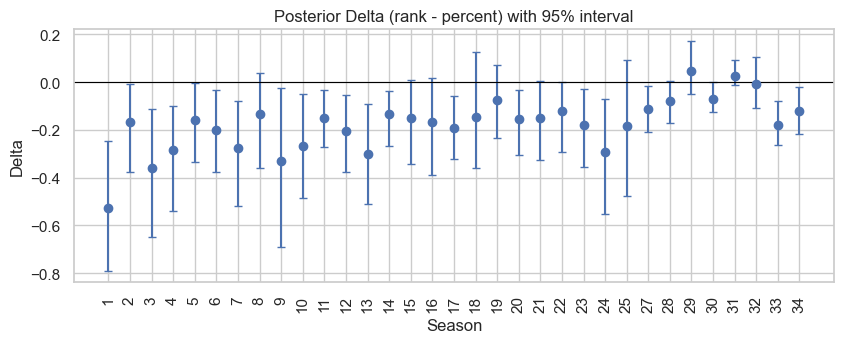
\includegraphics[width=\textwidth]{2_posterior_delta.png}
		\caption{\textbf{$\Delta_s$ (Rank$-$Percent).} $\Delta_s<0$ implies Percentage favors fan override.}
		\label{fig:posterior_delta}
	\end{minipage}
	\hfill
	\begin{minipage}{0.48\textwidth}
		\centering 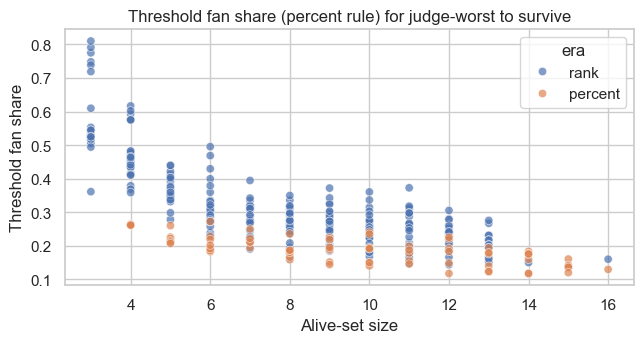
\includegraphics[width=0.95\textwidth]{2_threshold_fan_share.png}
		\caption{\textbf{Threshold Fan Share.} Required fan share for the judge-worst to survive.}
		\label{fig:threshold}
	\end{minipage}
\end{figure}

\paragraph{Explanation: Threshold Effect.}
Because percentage aggregation is linear while rank aggregation is stepwise, small judge-score gaps imply low fan-vote thresholds under the percentage rule but discrete penalties under the rank rule, accounting for the pattern in Fig.~\ref{fig:threshold}.








\subsection{Week-Level Analysis}
We model Season 28+ as \textbf{Bottom-2 + Judges' Save}:
\begin{equation}
	B_{s,t}=\text{arg\,two-min}_{i\in A_{s,t}} S_{i,s,t},\qquad 
	\hat e^{\mathrm{B2}}_{s,t}=\arg\min_{i\in B_{s,t}} J_{i,s,t},
\end{equation}
and quantify its effect by the \textbf{Reversal Rate}
\begin{equation}
	\mathrm{rev\_rate}_{s,t}=\Pr\!\left(\hat e^{\mathrm{B2}}_{s,t}\neq \hat e^{\mathrm{direct}}_{s,t}\right).
\end{equation}
Figure~\ref{fig:reversal_heatmaps} shows reversals concentrate late (Weeks 7--10) and are higher under \textbf{Percentage}, indicating stronger correction when vote magnitudes compress.

\begin{figure*}[ht]
	\centering
	\begin{minipage}{0.48\textwidth}
		\centering 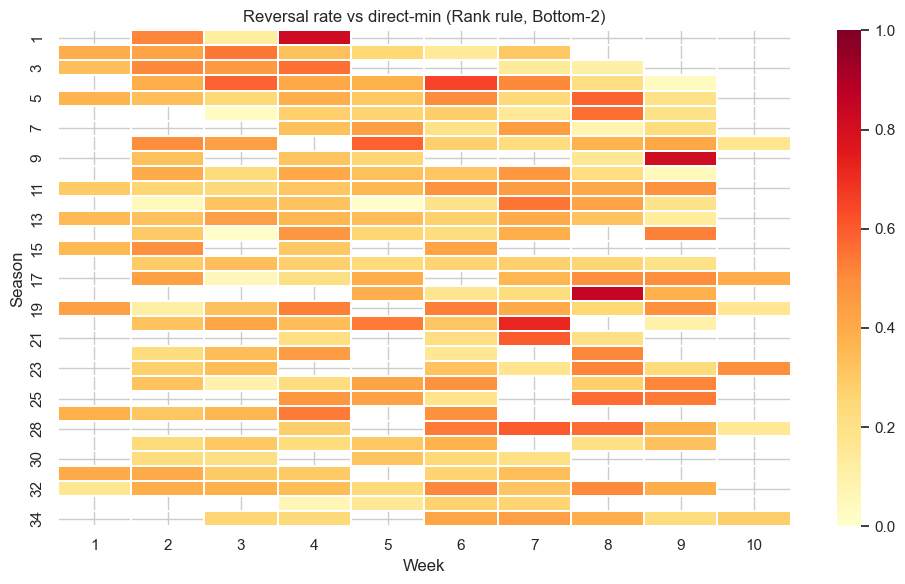
\includegraphics[width=\linewidth]{3_Reversal_Heatmap_Rank.png} \textbf{(a) Rank}
	\end{minipage}
	\hfill
	\begin{minipage}{0.48\textwidth}
		\centering 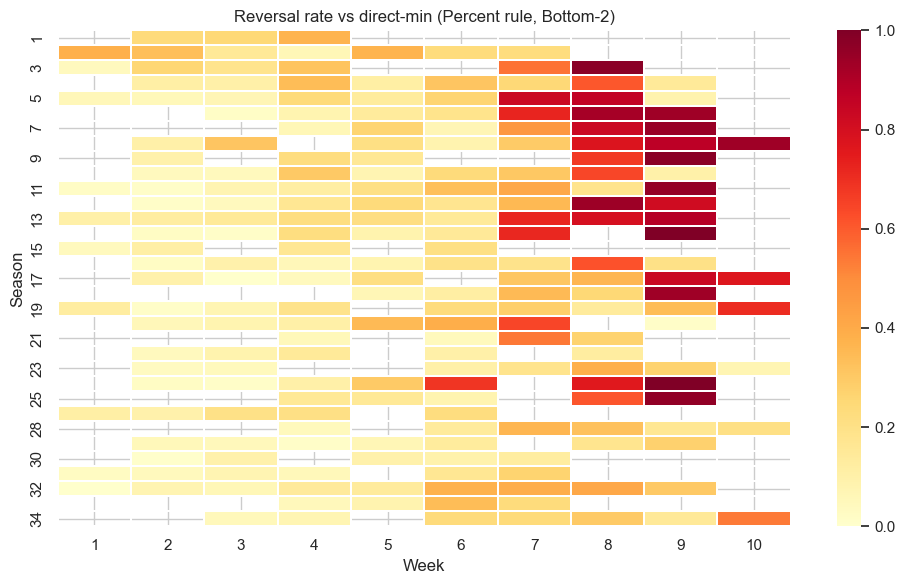
\includegraphics[width=\linewidth]{3_Reversal_Heatmap_Percent.png} \textbf{(b) Percentage}
	\end{minipage}
	\caption{\textbf{Reversal Heatmaps.} Darker cells indicate larger $\mathrm{rev\_rate}_{s,t}$.}
	\label{fig:reversal_heatmaps}
\end{figure*}







\subsection{Contestant-Level Case Studies}

\paragraph{Divergence Landscape:}
We locate fan-driven outliers using (i) rank disagreement $\Delta r_{i,s,t}=r^F_{i,s,t}-r^J_{i,s,t}$ and (ii) magnitude disagreement $\Delta s_{i,s,t}=\hat p_{i,s,t}-J_{i,s,t}$. Figure~\ref{fig:disagreement_landscape} shows that high-controversy contestant-weeks cluster in the top-left quadrant ($\Delta r\ll 0,\ \Delta s>0$), i.e., strong fan support despite weak judge evaluation.

\begin{figure}[htbp]
	\centering
	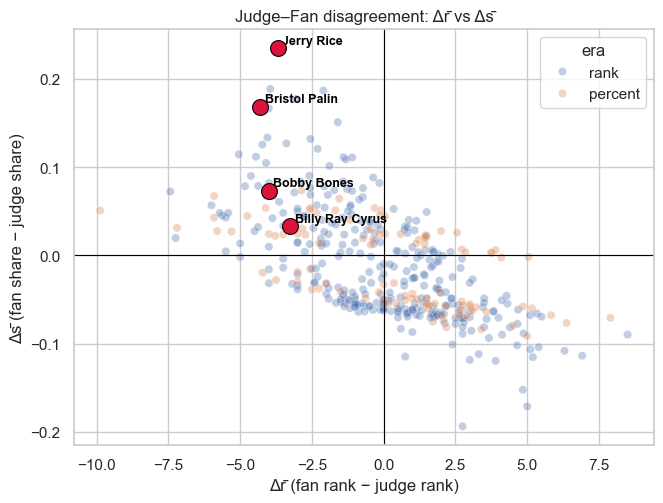
\includegraphics[width=0.60\linewidth]{3_Discrepancy_Scatter.png} 
	\caption{\textbf{Judge--Fan Disagreement Landscape.} Fan-driven controversies concentrate in the top-left quadrant ($\Delta r\ll 0,\ \Delta s>0$).}
	\label{fig:disagreement_landscape}
\end{figure}






\paragraph{Trajectory Simulation:}

We select six representative cases (Table \ref{tab:selected_cases}) based on maximum divergence ($|d|$) and their exposure to rule-based reversals (Flip Risk $> 0.2$). 


\begin{table}[ht]
	\centering
	\caption{\textbf{Selected Controversy Cases.} Cases selected from the top-left\& down-right quadrant of Fig \ref{fig:disagreement_landscape}.}
	\label{tab:selected_cases}
	\footnotesize
	\setlength{\tabcolsep}{3pt} 
	\begin{tabular}{llcc|llcc}
		\hline
		\textbf{S} & \textbf{Name} & \textbf{$|d|$} & \textbf{Flip} & \textbf{S} & \textbf{Name} & \textbf{$|d|$} & \textbf{Flip} \\
		\hline
		S2 & Jerry Rice & 3.69 & 0.87 & S27 & Bobby Bones & 4.00 & 0.57 \\
		S4 & B.R. Cyrus & 3.25 & 0.75 & S27 & Tinashe & 8.50 & 0.57 \\
		S11 & B. Palin & 4.30 & 0.97 & S31 & Vinny G. & 9.88 & 0.33 \\
		\hline
	\end{tabular}
\end{table}

\paragraph{Do Rank and Percentage yield the same outcome? No.}
Figure~\ref{fig:six_cases_grid} contrasts \textbf{Rank} and \textbf{Percentage} under direct elimination.
The left panels summarize week-level rule sensitivity and the implied survival curves, while the right panel compares judge and fan ranks and their aggregation under each rule.
Across cases, elimination trajectories frequently diverge, and the percentage rule systematically favors contestants with strong fan support when judge scores are close.
As a result, \textbf{Rank and Percentage do not always produce the same outcomes} for these contestants.


\paragraph{How does adding Bottom-2 + Judges' Save change results?}
Introducing the \textbf{Bottom-2 with Judges' Save} converts the rule into a \emph{conditional filter}: only contestants who repeatedly enter the Bottom-2 face judge veto. This produces an \textbf{asymmetric impact}:
(i) \textbf{fan-driven, judge-weak} contestants (e.g., Bobby Bones, Vinny G.) are more frequently exposed to Bottom-2 and thus experience \textbf{reduced survival}, while
(ii) \textbf{technical leaders} (e.g., Tinashe) rarely fall into Bottom-2 and are therefore \textbf{largely unaffected}.
Overall, the Save mechanism dampens extreme fan-driven persistence \emph{without} broadly altering outcomes for consistently strong performers.

% --- 定义 ContestantBlock 命令 ---
\newcommand{\ContestantBlock}[3]{%
	\begin{minipage}[t]{0.48\linewidth}
		\centering
		{\scriptsize \textbf{S#3: #2}} \vspace{1pt} \\
		\begin{minipage}[c]{0.42\linewidth}
			\includegraphics[width=\linewidth]{4_EliminationProbability_#1.png} \\[-2pt]
			\includegraphics[width=\linewidth]{4_SurvivalCurves_#1.png}
		\end{minipage}%
		\hfill
		\begin{minipage}[c]{0.56\linewidth}
			\includegraphics[width=\linewidth]{4_RankVsPercentage_#1.png}
		\end{minipage}
	\end{minipage}%
}
% ---------------------------------

\begin{figure*}[ht]
	\centering
	\setlength{\tabcolsep}{1pt}
	\ContestantBlock{BillyRayCyrus}{Billy Ray Cyrus}{4} \hfill \ContestantBlock{JerryRice}{Jerry Rice}{2} \\[0.2cm]
	\ContestantBlock{BristolPalin}{Bristol Palin}{11} \hfill \ContestantBlock{BobbyBones}{Bobby Bones}{27} \\[0.2cm]
	\ContestantBlock{Tinashe}{Tinashe}{27} \hfill \ContestantBlock{VinnyGuadagnino}{Vinny G.}{31}
	\caption{\textbf{Contestant Trajectories.} Left sub-panels show Survival Probability (Solid=Save, Dashed=Direct); Right sub-panels show rank divergence.}
	\label{fig:six_cases_grid}
\end{figure*}














\subsection{Systemic Analysis}


We summarize season-level stability with a \textbf{Mechanism Phase Diagram} (Fig.~\ref{fig:phase_diagram}). Each season is embedded by \textbf{fan influence} on the x-axis, $\mu(|\Delta s|)$ (the magnitude of the popularity cushion), and \textbf{judge consistency} on the y-axis, $1-\mu(|\Delta r|)$ (how aligned eliminations are with judge ranking). Points represent four mechanisms (Pct/Rank $\times$ Direct/Bottom-2+Save), and arrows trace the same season under different rules.

Two patterns are clear. First, moving from \textbf{Direct} to \textbf{Bottom-2+Save} produces an upward shift in y (higher judge consistency) with only modest change in x, i.e., a near-\emph{vertical lift} in technical fidelity. Second, in high fan-influence seasons ($\mu(|\Delta s|)\gtrsim 0.3$), the \textbf{Pct+Direct} mechanism is most exposed to low-fidelity outcomes, while \textbf{Pct+Bottom-2} remains high on y, indicating effective tail-risk control without suppressing the fan signal.

\begin{figure}[ht]
	\centering
	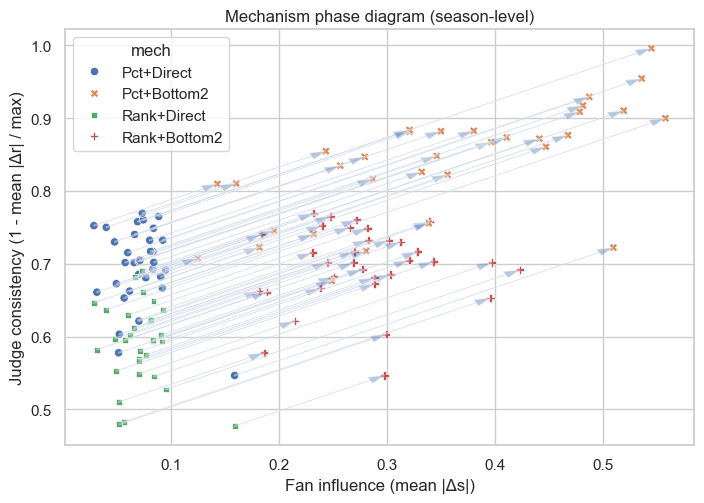
\includegraphics[width=0.60\linewidth]{5_Mechanism phase diagram.png}
	\caption{\textbf{Mechanism Phase Diagram (season-level).} x: fan influence $\mu(|\Delta s|)$; y: judge consistency $1-\mu(|\Delta r|)$. Arrows show within-season shifts across mechanisms; Bottom-2+Save yields a near-vertical improvement in technical fidelity.}
	\label{fig:phase_diagram}
\end{figure}

\paragraph{Recommendation.} Although \textbf{Rank} can be more protective of \emph{low-popularity} contestants by down-weighting vote magnitudes, that same \emph{magnitude neglect} also makes the system less faithful when fan support is highly concentrated (it caps both extremes). We therefore recommend \textbf{Percentage} as the base rule to preserve the true intensity of audience preference, but \emph{pair it} with \textbf{Bottom-2 + Judges' Save} as a conditional safety filter. As Fig.~\ref{fig:phase_diagram} shows, this hybrid yields a near-vertical gain in judge consistency (technical fidelity $\uparrow$) with little change in fan influence, i.e., it keeps the democratic signal while clipping the tail risk of fan-driven distortions in high-entropy seasons.









\section{Problem 3: Survival Determinant Analysis}

To quantify the drivers of survival, we constructed a multi-stage econometric framework to decouple \textbf{Technical Survival} (Judge-driven) from \textbf{Popularity Survival} (Fan-driven).

\subsection{Demographic Divergence}

We strictly distinguish between two evaluation metrics: $Y^{\text{Judge}}$ (Technical Score) and $Y^{\text{Fan}}$ (Popularity Vote). We employ parallel OLS regressions to estimate the marginal effect of Age and Industry:
\begin{equation} \label{eq:demo_model}
	Y_{i,t}^{\text{type}} = \alpha + \beta_{Age}^{\text{type}} \cdot \text{Age}_i + \sum_{k} \delta_{k}^{\text{type}} \cdot \mathbb{I}(\text{Industry}_i = k) + \epsilon_{i,t}
\end{equation}
\noindent \textit{Metric Definition:} $Y_{i,t}$ denotes the standardized outcome; $\beta_{Age}$ captures the biological penalty; $\delta_{k}$ represents the industry-specific bias relative to the baseline.

\begin{figure}[htbp]
	\centering
	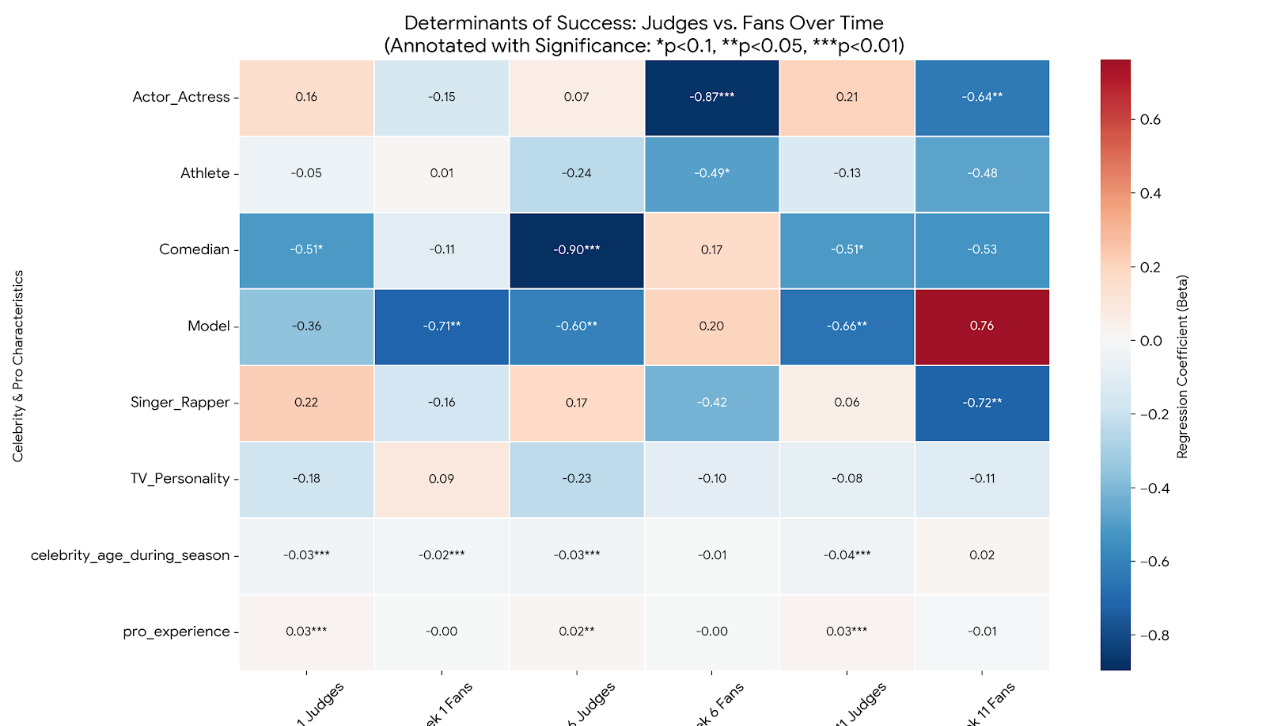
\includegraphics[width=0.95\linewidth]{6_Success_Factors_Judges_vs_Fans.png}
	\caption{\textbf{Temporal Evolution of Preferences.} Heatmap of regression coefficients from Eq. \ref{eq:demo_model} across stages ($W1, W6, W11$). \textbf{Red/Blue} indicates significant advantage/penalty ($p<0.05$).}
	\label{fig:demographics}
\end{figure}

\noindent \textbf{Analysis of Divergence (Figure \ref{fig:demographics}):}
\begin{itemize}
	\item \textbf{Industry Effect (The Expectation Trap):} \textit{Actors} face a drastic sentiment reversal. Initially rewarded by Judges ($W1: \beta \approx 0.16$), they suffer a severe Fan penalty by mid-season ($W6: \beta = -0.87^{*}$). This confirms "Audience Fatigue": high initial expectations decay rapidly if not met with constant growth.
	\item \textbf{Age Effect (The Underdog Arc\textsuperscript{\cite{paharia2011}}):}
	Judges consistently penalize physical decline ($\beta \approx -0.04^{*}$ across all weeks). 
	In contrast, fan penalties vanish by $W6$ and reverse by $W11$. 
	Fans transition from evaluating capability to rewarding resilience.


\end{itemize}


\subsection{Professional Partner Effects}

We investigate whether a partner's influence stems from \textbf{Historical Ability} ($H_{abil}$) or \textbf{Institutional Tenure} ($H_{exp}$).
\begin{equation}
	H_{abil} = \text{Avg}(\text{Rank}_{p, \text{past}}), \quad H_{exp} = \sum \mathbb{I}(s \in S_p)
\end{equation}

To isolate the partner's intrinsic "value-add" independent of the celebrity's skill, we fit a \textbf{Fixed Effects Model}:
\begin{equation} \label{eq:fe_model}
	Z_{i,t}^{\text{Judge}} = \mu + \gamma_1 H_{abil} + \gamma_2 H_{exp} + \mathbf{\alpha_p} + \epsilon_{i,t}
\end{equation}
where $\mathbf{\alpha_p}$ represents the partner-specific fixed effect.

\paragraph{Mechanism Identification:}
Figure \ref{fig:partner_heatmap} resolves the influence pathway, while Figure \ref{fig:partner_scatter_bar} quantifies individual efficacy.

\begin{figure}[htbp]
	\centering
	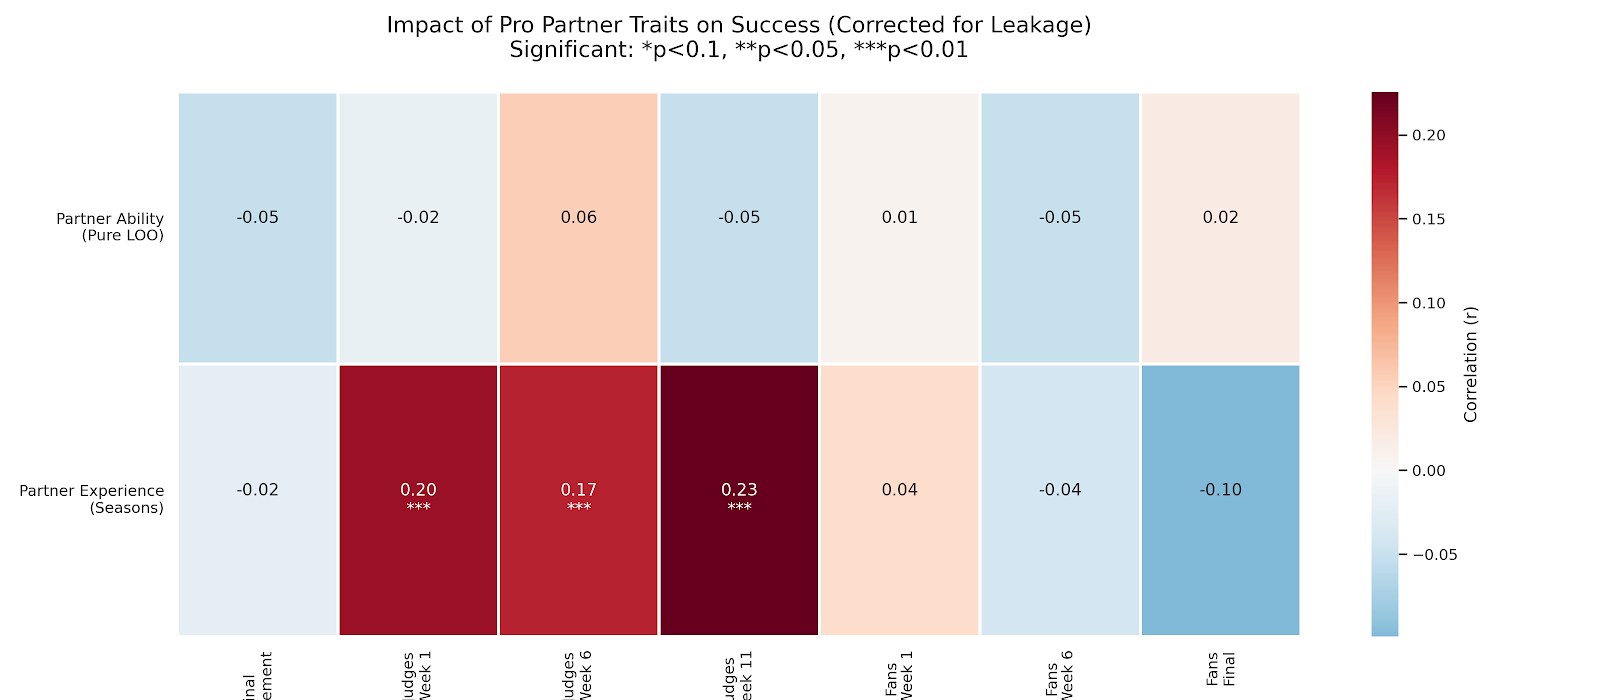
\includegraphics[width=0.95\linewidth]{6_Partner_Traits_Correlation.png}
	\caption{\textbf{Correlation Heatmap:} Partner Tenure ($H_{exp}$) correlates significantly with Judge Scores ($r=0.23^{*}$) but has near-zero correlation with Fan Votes, proving experience targets technical scoring.}
	\label{fig:partner_heatmap}
\end{figure}

\begin{figure}[htbp]
	\centering
	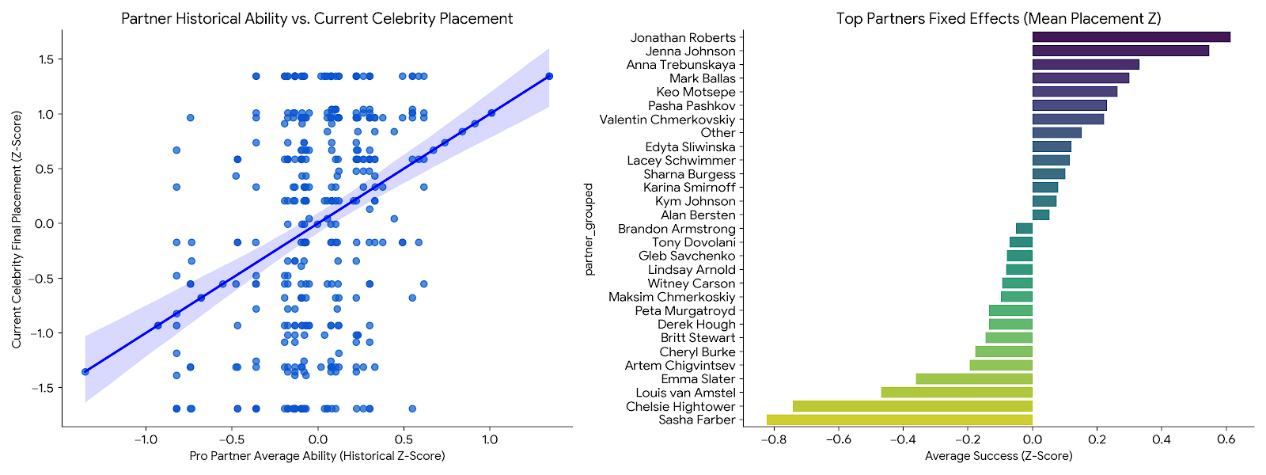
\includegraphics[width=0.95\linewidth]{6_Pro_Partner_Historical_Impact.png}
	\caption{\textbf{Partner Heterogeneity:} (Left) Raw ability ($H_{abil}$) shows noisy correlation. (Right) Fixed effects $\mathbf{\alpha_p}$ derived from Eq. \ref{eq:fe_model} identify "Kingmaker" partners who systematically lift performance.}
	\label{fig:partner_scatter_bar}
\end{figure}

\noindent \textbf{Analysis:}
The heatmap (Fig. \ref{fig:partner_heatmap}) proves that Veteran partners do not generate direct popularity. Instead, the Fixed Effects ranking (Fig. \ref{fig:partner_scatter_bar}, Right) confirms they function as a \textbf{Technical Safety Net} ($\alpha_p > 0$), optimizing scoring strategies to protect celebrities from elimination.


\subsection{Dynamic Interaction Modeling}

Static factors explain the baseline, but longevity is driven by growth. We define \textbf{Surprise index}  \textsuperscript{\cite{burgoon1993}}($\mathcal{S}_i$) and \textbf{Vote Growth} ($\mathcal{G}_i$) as:
\begin{equation}
	\mathcal{S}_i = Z_{\text{Judge}, t} - Z_{\text{Fan}, t-1}, \qquad \mathcal{G}_i = Z_{\text{Fan}, t} - Z_{\text{Fan}, t-1}
\end{equation}

To test for viral effects, we fit a quadratic interaction model:
\begin{equation} \label{eq:growth_model}
	\mathcal{G}_i = \beta_0 + \beta_1 \mathcal{S}_i + \underbrace{\beta_2 \mathcal{S}_i^2}_{\text{Viral Convexity}} + \underbrace{\beta_3 (\mathcal{S}_i \times H_{exp})}_{\text{Tenure Leverage}} + \epsilon
\end{equation}

\begin{figure}[htbp]
	\centering
	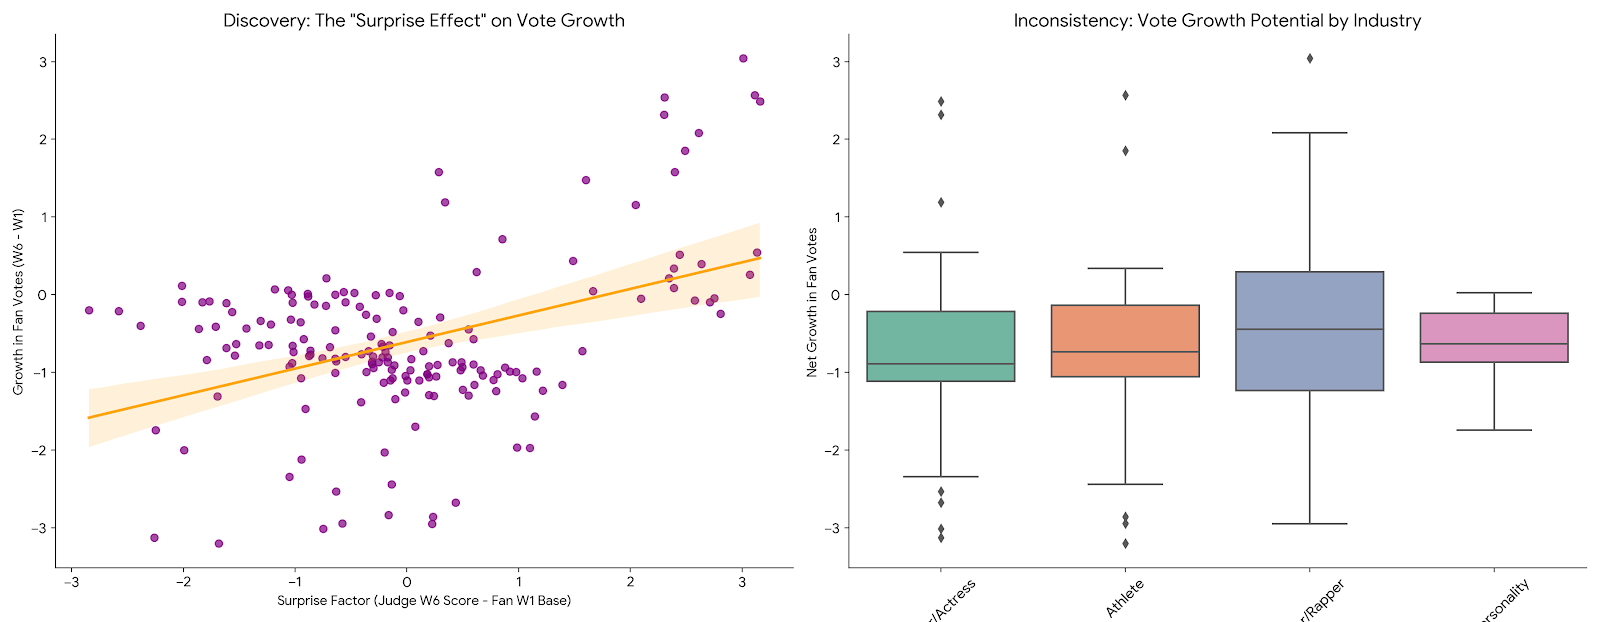
\includegraphics[width=0.95\linewidth]{6_Surprise_Effect_Vote_Growth.png}
	\caption{\textbf{Linear Response:} Positive slope ($\beta_1=0.34, p<0.001$) confirms "beating expectations" drives votes. Athletes (Green) show highest conversion rates.}
	\label{fig:surprise_linear}
\end{figure}

\begin{figure}[htbp]
	\centering
	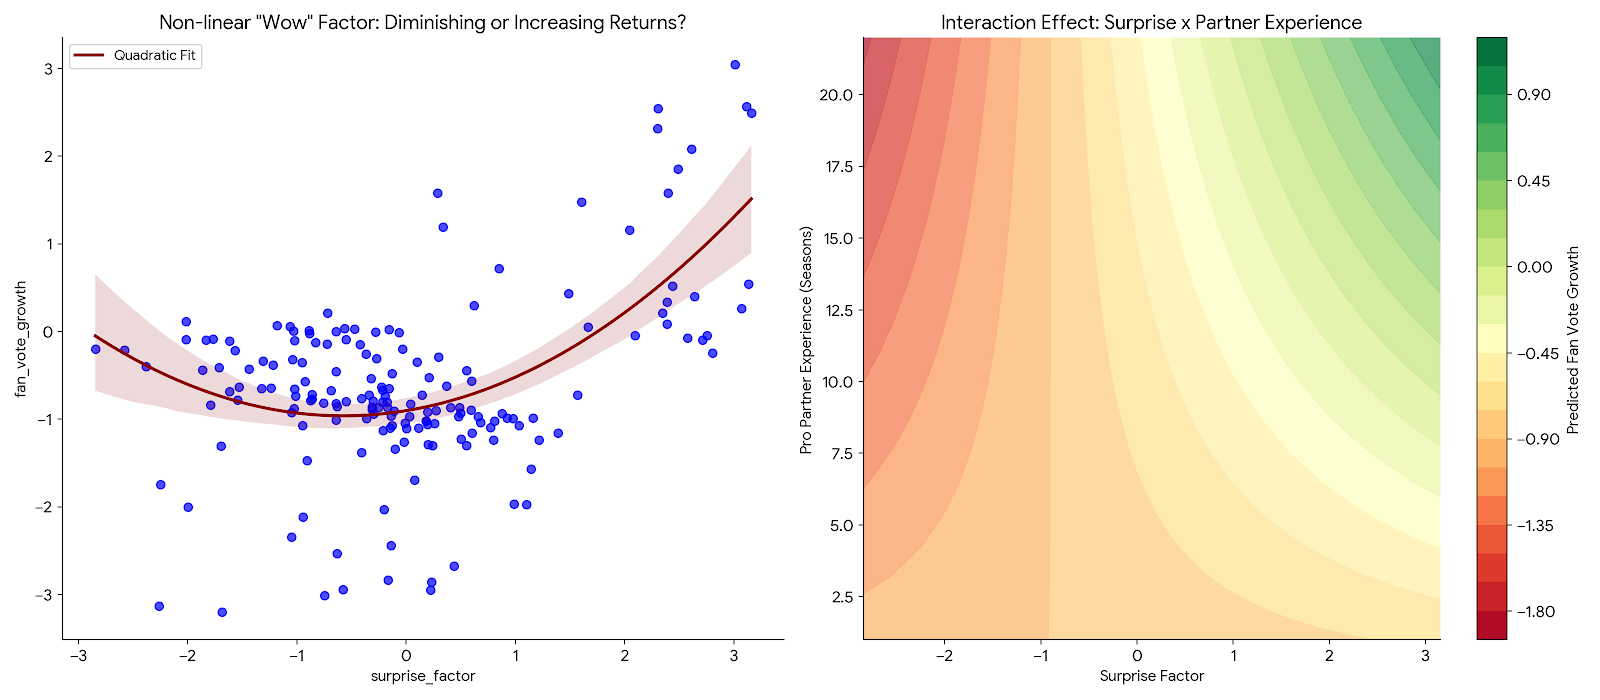
\includegraphics[width=0.95\linewidth]{6_Surprise_NonLinearity_and_Interaction.png}
	\caption{\textbf{Non-Linear Mechanics:} (Left) Positive quadratic term $\beta_2$ indicates exponential returns. (Right) Interaction term $\beta_3 > 0$: Veteran partners amplify the vote yield from a given Surprise.}
	\label{fig:surprise_nonlinear}
\end{figure}

\noindent \textbf{Growth Mechanics (Figures \ref{fig:surprise_linear} \& \ref{fig:surprise_nonlinear}):}
\begin{itemize}
	\item \textbf{The Matthew Effect \textsuperscript{\cite{merton1968}}($\beta_2 > 0$):} The upward curve (Fig. \ref{fig:surprise_nonlinear}, Left) indicates increasing marginal returns. Small surprises yield linear growth, but massive surprises trigger viral vote spikes.
	\item \textbf{Leverage Effect ($\beta_3 > 0$):} The interaction heatmap (Fig. \ref{fig:surprise_nonlinear}, Right) reveals that Veteran Partners are multipliers. For the same level of $\mathcal{S}_i$, partners with high tenure ($H_{exp}$) extract significantly higher vote growth, confirming superior narrative management.
\end{itemize}


\subsection{Summary of Determinants}

\begin{enumerate}
	\item \textbf{Demographics.}
	Judges act as relatively static filters, imposing age-related penalties, whereas fans respond dynamically by penalizing perceived entitlement (fatigue) while rewarding redemption narratives for aging underdogs.
	\item \textbf{Partners.}
	Partner tenure ($H_{exp}$) emerges as a decisive factor, not by directly generating popularity, but by creating a \textbf{technical safety net} (high $\alpha_p$) through Eq.~\ref{eq:fe_model}.
	\item \textbf{Growth.}
	Seasonal longevity is sustained by \textbf{surprise}, with a nonlinear response (Eq.~\ref{eq:growth_model}) that is amplified by partner tenure, translating technical improvement into outsized political capital.
\end{enumerate}




\section{Problem 4: Mechanism Design and Optimization}

In a commercial competition, perfect fairness is neither attainable nor desirable; we therefore balance \textbf{legitimacy} and \textbf{engagement}. We formalize this trade-off with two criteria: \emph{fairness} (limit extreme individual injustice) and \emph{excitement} (retain fan agency), and propose two rules: \textbf{V1} (bottom-3 judge gate + fan save) for excitement, and \textbf{V2} (tempered fan shares + bounded merit/momentum bonuses + bottom-2 judges' save) for fairness with suspense. Because true fan votes are unobserved, we evaluate both via Monte-Carlo season simulations using posterior fan-share draws from Problem~1 (fixed seeds for reproducibility).


\subsection{Optimization Objectives}
We design weekly vote rules that balance the show’s core tension: \textbf{judges} signal technical merit, while \textbf{fans} provide agency.

\paragraph{Interpretation of Fairness:}
A system is considered fair if it rarely eliminates a judge-strong couple, thereby minimizing severe injustice.\textsuperscript{\cite{rawls1971}}
We quantify this using the \emph{technical shock} rate
\begin{equation}
	\text{Shock}_k=\Pr\!\left(\text{elim}(s,t)\in \text{Top-}k \text{ by judges at week }(s,t)\right),
\end{equation}
which should remain small.

\paragraph{Interpretation of Excitement:}
A system is considered exciting if fan votes can materially alter weekly survival paths rather than merely perturb rankings, while retaining credibility through a judge gate or a judges’ save.


\paragraph{Why simulation?}
True fan votes are unobserved, so rule quality cannot be supervised directly. We therefore evaluate proposed rules with a Monte-Carlo season simulator driven by posterior fan-share draws from Problem~1, $\pi^{(b)}_{i,s,t}$, producing elimination paths and placements under uncertainty (fixed seeds for reproducibility).




\subsection{Mechanism I: Fan-Determined Elimination with a Judge Gate}

\noindent\textbf{Design intent:} maximize \emph{fan agency}---fans directly decide who leaves each week---while using judges only to define a credible at-risk set.

For each non-final week $(s,t)$ with alive set $A_{s,t}$, judges nominate the bottom-$K$ couples ($K=3$):
\begin{equation}
B^{J}_{s,t}=\arg\,\text{K-min}_{i\in A_{s,t}} J_{i,s,t},
\end{equation}
then fans eliminate the least-supported within this set:
\begin{equation}
e_{s,t}=\arg\min_{i\in B^{J}_{s,t}} p_{i,s,t},
\end{equation}
where $p_{i,s,t}$ is supplied by posterior draws $p^{(b)}_{i,s,t}$ from Problem~1. The finale remains unchanged (placements by combined-score ranking).

To isolate \emph{when} this rule matters, we split weeks into \emph{early} ($|A_{s,t}|>m$) vs.\ \emph{late} ($|A_{s,t}|\le m$, non-final; $m=8$) and compare three controlled variants: (S1) baseline all season, (S2) late-stage-only activation, and (S3) full-season activation (finale fixed).


\paragraph{Large-Sample Validation:}
We stratify contestants into three archetypes using season-level judge--fan disagreement (aggregated $\Delta r_{i,s,t}=r^F_{i,s,t}-r^J_{i,s,t}$ and $\Delta s_{i,s,t}$): top 25\% \textbf{Popularity-type}, bottom 25\% \textbf{Technical-type}, and middle 50\% \textbf{Balanced}. We then compare Monte-Carlo outcomes across schemes.

Figure~\ref{fig:delta_avg_rank_S3_S1} shows that the intervention shifts \emph{conditional} average placements in some weeks (positive $\Delta$ indicates improved rank), but Figure~\ref{fig:survival_by_archetype} shows only \emph{modest} changes in unconditional survival: Balanced is nearly unchanged, Popularity-type remains advantaged overall, and any gains for Technical-type are limited. Thus, the mechanism mainly supports \textbf{excitement} (fan-driven eliminations within the gate) while delivering only \textbf{partial fairness} improvement at the population level.



\begin{figure}[htbp]
	\centering
	\begin{minipage}{0.47\linewidth}
		\centering
		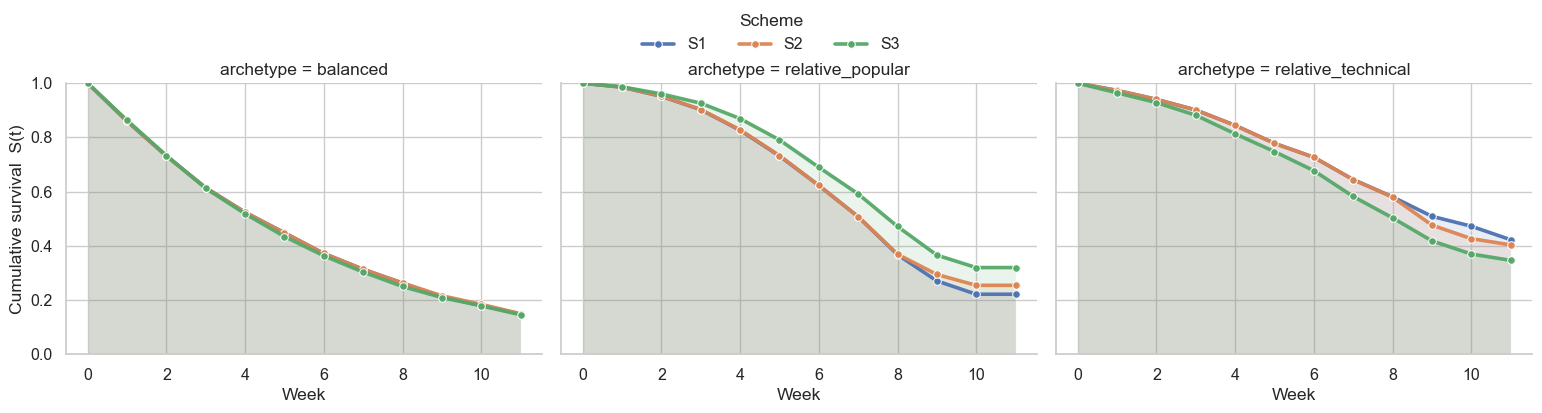
\includegraphics[width=\linewidth]{8_V1_plot1.png}
		\caption{\textbf{$\Delta$ Average Rank (S3$-$S1).} Week-by-archetype heatmap of $\Delta(-\overline{\mathrm{rank}})=(-\overline{\mathrm{rank}}_{\mathrm{S3}})-(-\overline{\mathrm{rank}}_{\mathrm{S1}})$; positive values indicate improved average placement. Black lines show the weekly mean effect by archetype.}
		\label{fig:delta_avg_rank_S3_S1}
	\end{minipage}
	\hspace{0.03\linewidth}
	\begin{minipage}{0.47\linewidth}
		\centering
		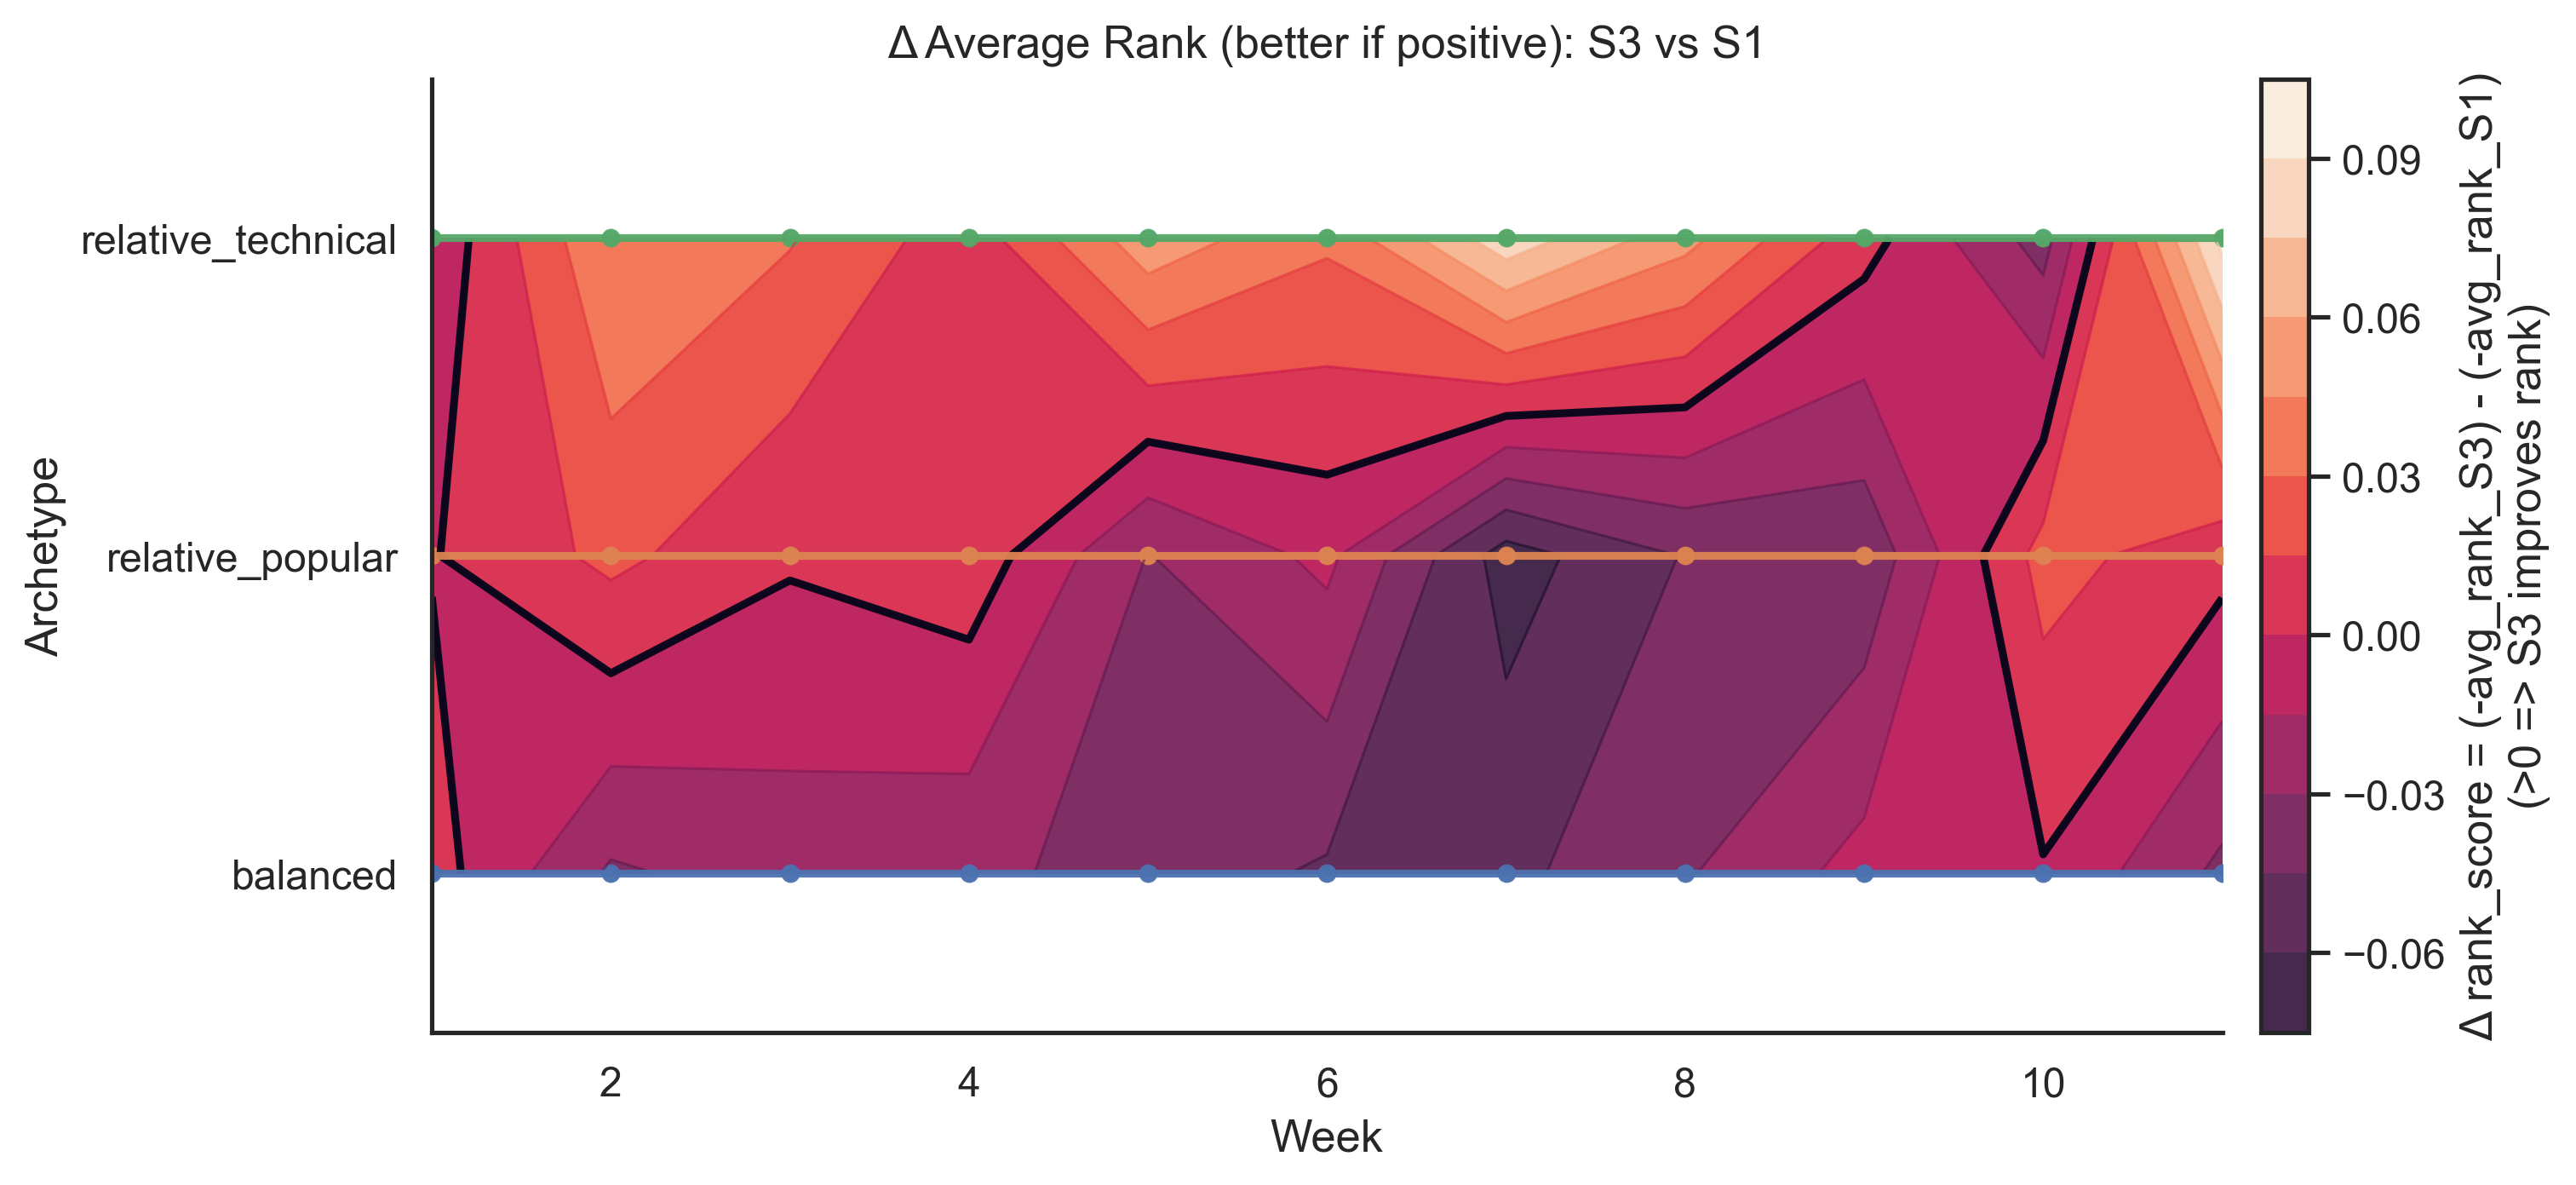
\includegraphics[width=\linewidth]{8_fig_diff_contour_avg_rank_S3_minus_S1.png}
		\caption{\textbf{Cumulative Survival by Archetype and Scheme.} Survival function $S(t)$ across weeks for three archetypes under schemes S1--S3, summarizing the fraction remaining at or beyond week $t$.}
		\label{fig:survival_by_archetype}
	\end{minipage}
\end{figure}


\paragraph{Controversial Contestant Case Studies:}
We examine historically controversial contestants with large judge--fan divergence and, over posterior draws, summarize their bottom-$K$ nomination rates, scheme-specific elimination probabilities, and reversal frequencies.

Across the highlighted cases (Jerry Rice, Billy Ray Cyrus, Bristol Palin, Bobby Bones), the mechanism \textbf{does not correct} the canonical controversy: they still survive deep into the season despite weak judge signals, and the judge--fan gap can even widen. The reason is structural---bottom-$K$ exposure is largely governed by fan support, so highly popular contestants rarely enter the risk set where judge-based corrections can operate, effectively creating \textbf{pre-filter immunity}.









\subsection{Mechanism II: Hybrid Momentum Model}
V1 maximizes fan agency but, in simulation, still allows highly popular yet technically weak contestants (including the canonical controversial cases) to advance deep. V2 targets this failure while preserving suspense by (i) tempering fan influence with diminishing returns, (ii) boosting technical merit via a unit-free shape adjustment, (iii) adding a bounded short-memory improvement bonus, and (iv) applying a Bottom-2 judges' save as a safety valve against severe technical injustice.

V2 preserves fairness while maintaining suspense by damping extreme popularity, sharpening technical separation, adding a capped improvement bonus, and applying a Bottom-2 judges’ save.

\textbf{Fan support }is first tempered on the simplex to impose diminishing returns on extreme popularity,
\begin{equation}
	\tilde p_{i,s,t}=\frac{p_{i,s,t}^{\gamma}}{\sum_{k\in A_{s,t}}p_{k,s,t}^{\gamma}},\qquad 0<\gamma\le1 .
\end{equation}
When $\gamma<1$, the transformation compresses the head and lifts the tail while remaining nonnegative and summing to one, unlike a log transform.

\textbf{Technical merit} is then sharpened in a unit-free manner by reweighting judge scores,
\begin{equation}
	\tilde J_{i,s,t}=\frac{J_{i,s,t}^{\delta}}{\sum_{k\in A_{s,t}}J_{k,s,t}^{\delta}},\qquad \delta\ge1 .
\end{equation}
Values $\delta>1$ increase separation among top technical performers without introducing ad-hoc point bonuses.

To reward recent improvement without granting immunity, we introduce a bounded, short-memory \textbf{momentum term}.
Let $m_{i,s,t}=T_{i,s,t}-\frac{1}{L}\sum_{\ell=1}^{L}T_{i,s,t-\ell}$, standardize it to $z_{i,s,t}$, and define
\begin{equation}
	B_{i,s,t}=\mu\cdot \tanh\!\left(\frac{z_{i,s,t}}{c}\right),
\end{equation}
so that improvement is beneficial but saturates (typically with $L\in\{2,3\}$).

These components are combined into a single score, followed by a Bottom-2 judges’ save mechanism:
\begin{equation}
	S_{i,s,t}=w_J\,\tilde J_{i,s,t}+w_F\,\tilde p_{i,s,t}+B_{i,s,t},\qquad w_J+w_F=1,
\end{equation}
\begin{equation}
	\text{Bottom2}(s,t)=\arg\,\text{two-min}_{i\in A_{s,t}} S_{i,s,t},\qquad
	\text{elim}(s,t)=\arg\min_{i\in \text{Bottom2}(s,t)} T_{i,s,t}.
\end{equation}
Under this rule, fan votes determine which contestants enter danger, while judges decide the final exit, thereby limiting severe technical injustice.

Throughout, we use the default parameters
$w_J=0.80,\;w_F=0.20,\;\gamma=0.45,\;\delta=1.35,\;\mu=0.01$ (with fixed $c$), and $L\in\{2,3\}$.





\begin{figure}[htbp]
	\centering
	
	% ---------- Left panel ----------
	\begin{minipage}[t]{0.48\textwidth}
		\centering
		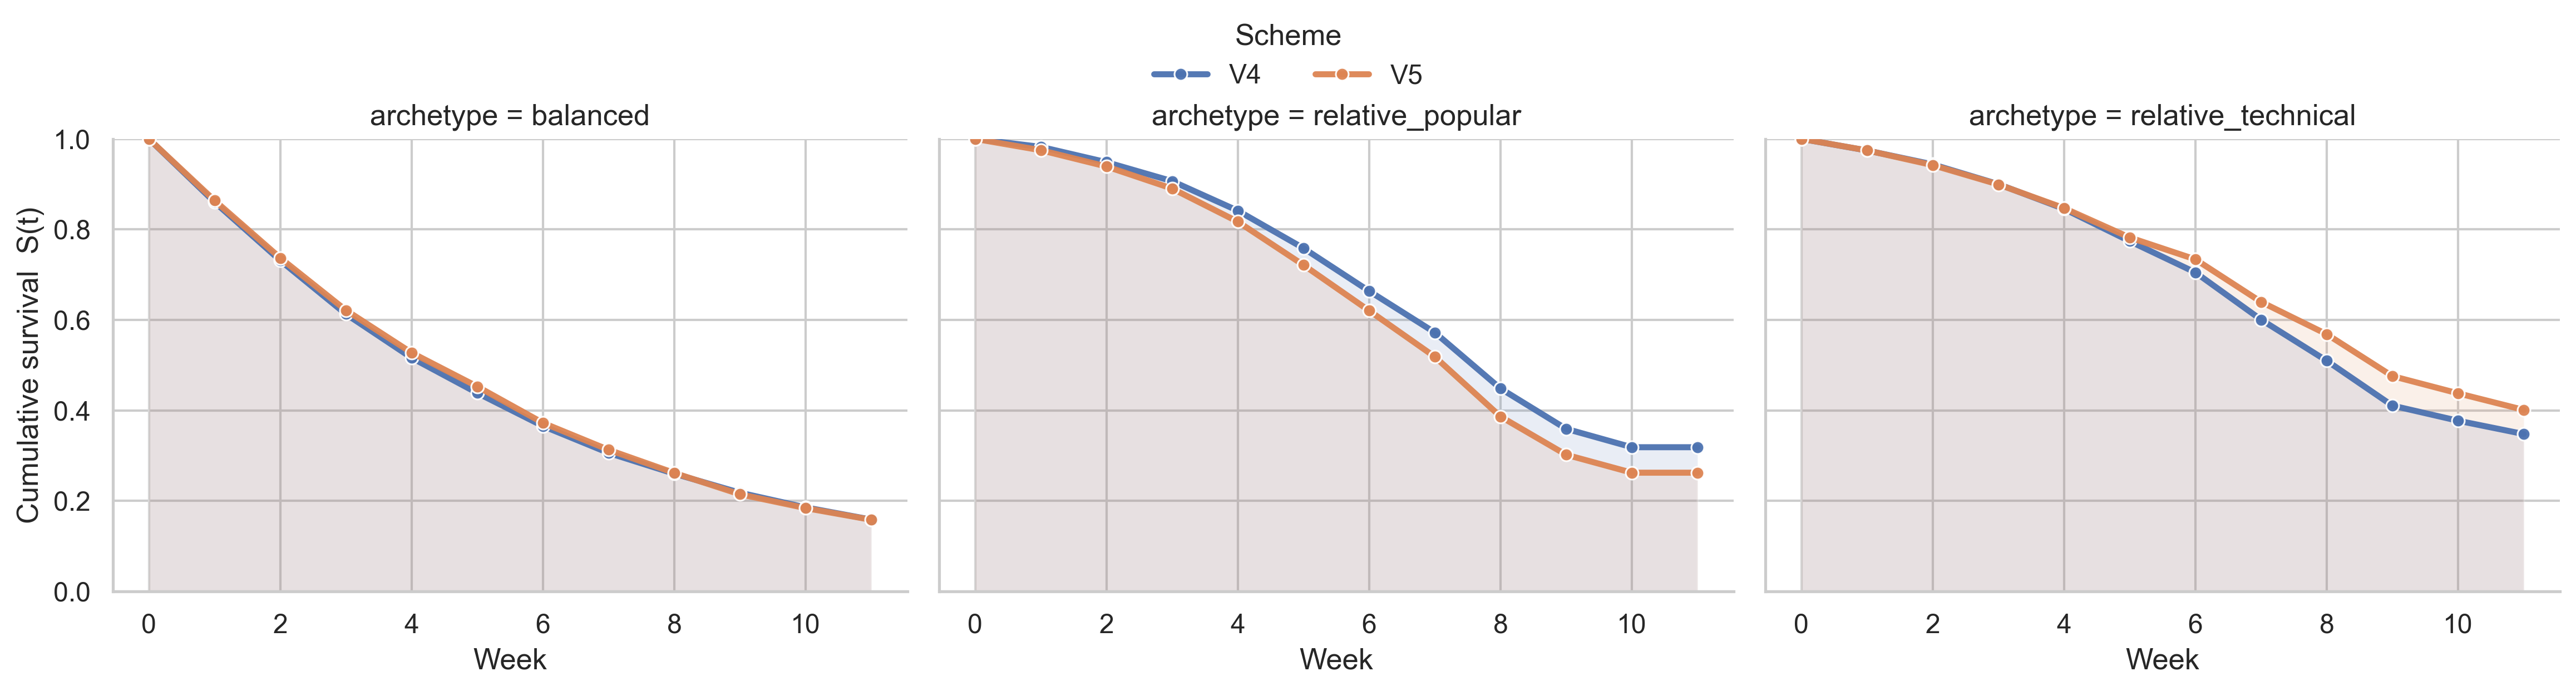
\includegraphics[width=\linewidth]{8_fig_ribbon_survival_by_archetype.png}
		
		\vspace{0.3em}
		{\small \textbf{(a)} \textbf{Archetype-level cumulative survival (Baseline V0 vs V2):}
			Curves show the unconditional survival function $S(t)$ across weeks for each archetype; larger $S(t)$ means a higher fraction of contestants remain in the competition (deeper runs).}
		
	\end{minipage}
	\hfill
	% ---------- Right panel ----------
	\begin{minipage}[t]{0.48\textwidth}
		\centering
		
		\setlength{\tabcolsep}{2pt} % horizontal padding
		\renewcommand{\arraystretch}{1.0}
		
		\begin{tabular}{ccc}
			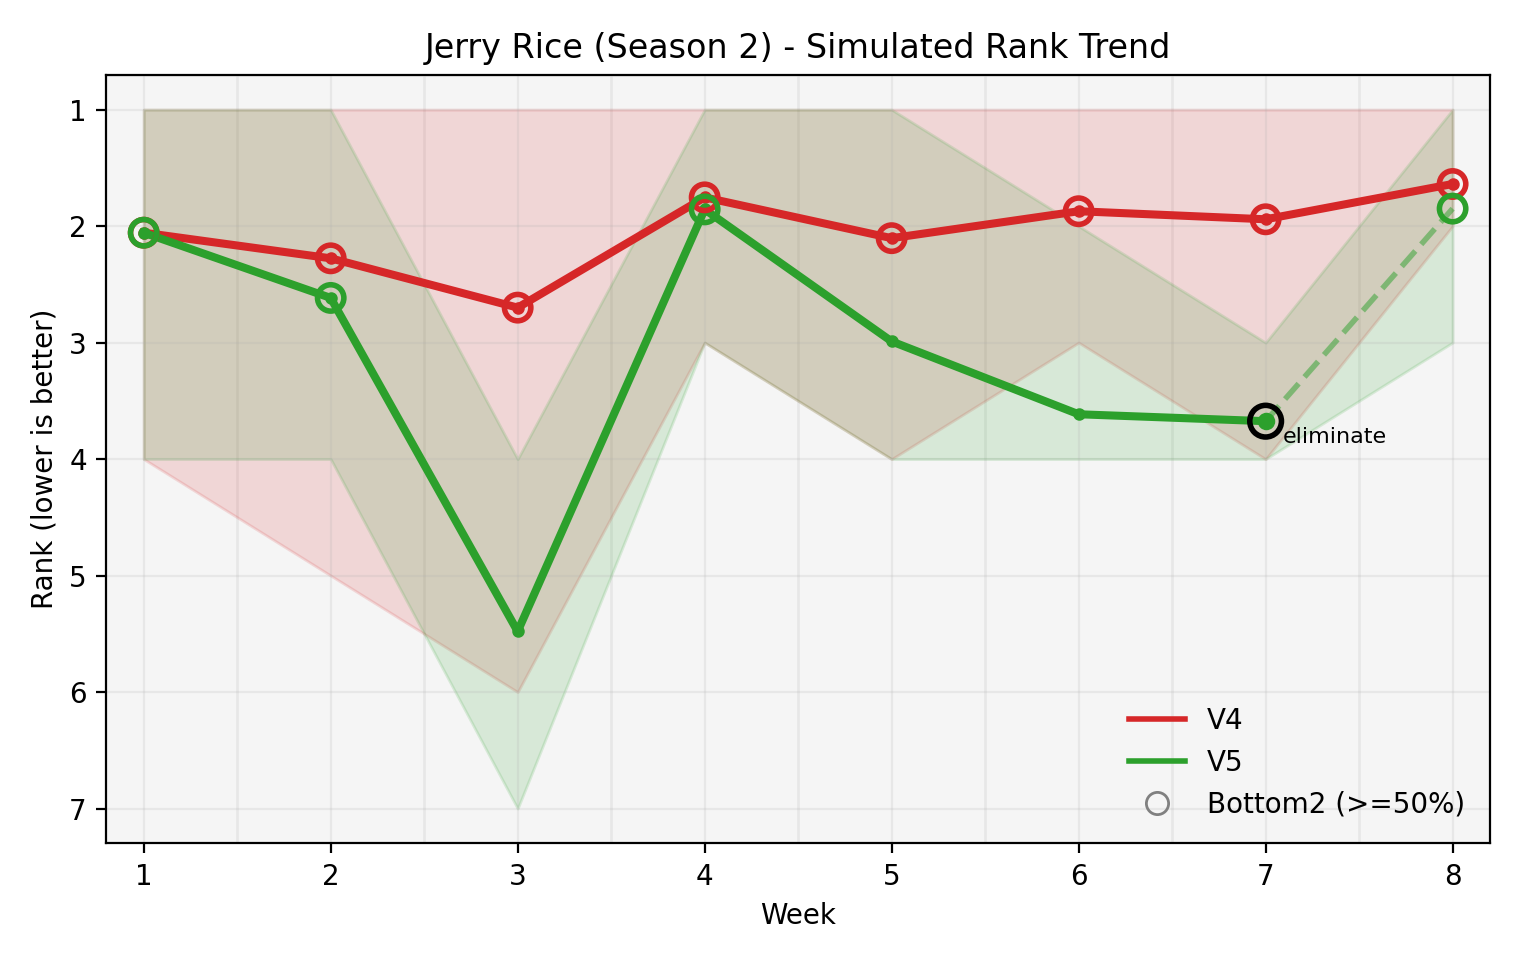
\includegraphics[width=0.32\linewidth]{8_fig_sim2_trend_2_Jerry_Rice.png} &
			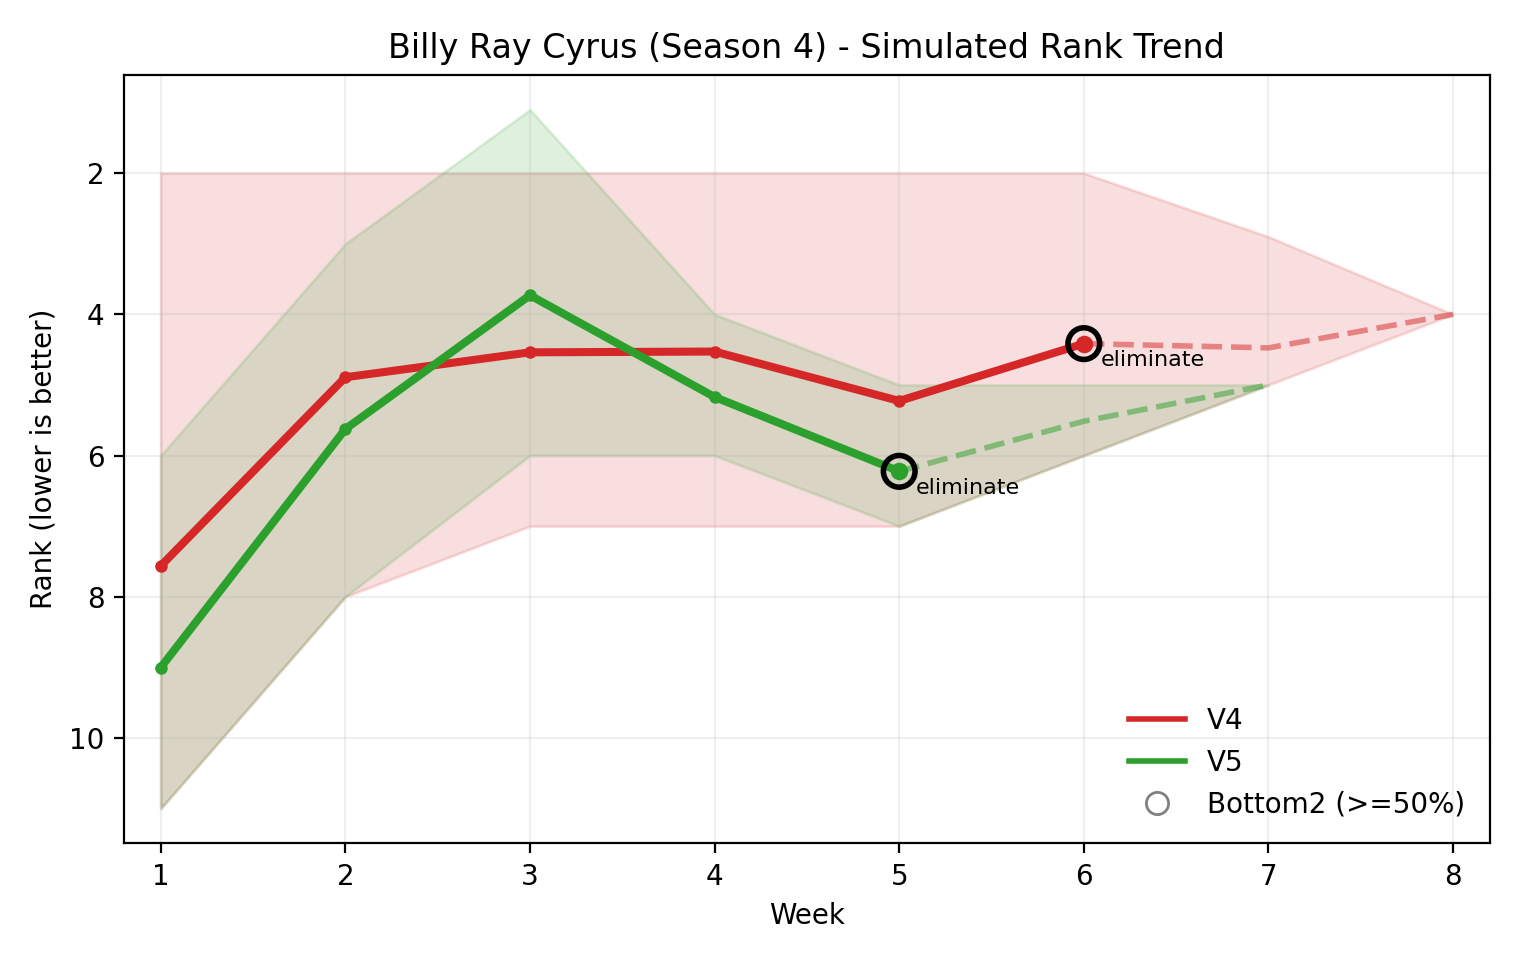
\includegraphics[width=0.32\linewidth]{8_fig_sim2_trend_4_Billy_Ray_Cyrus.png} &
			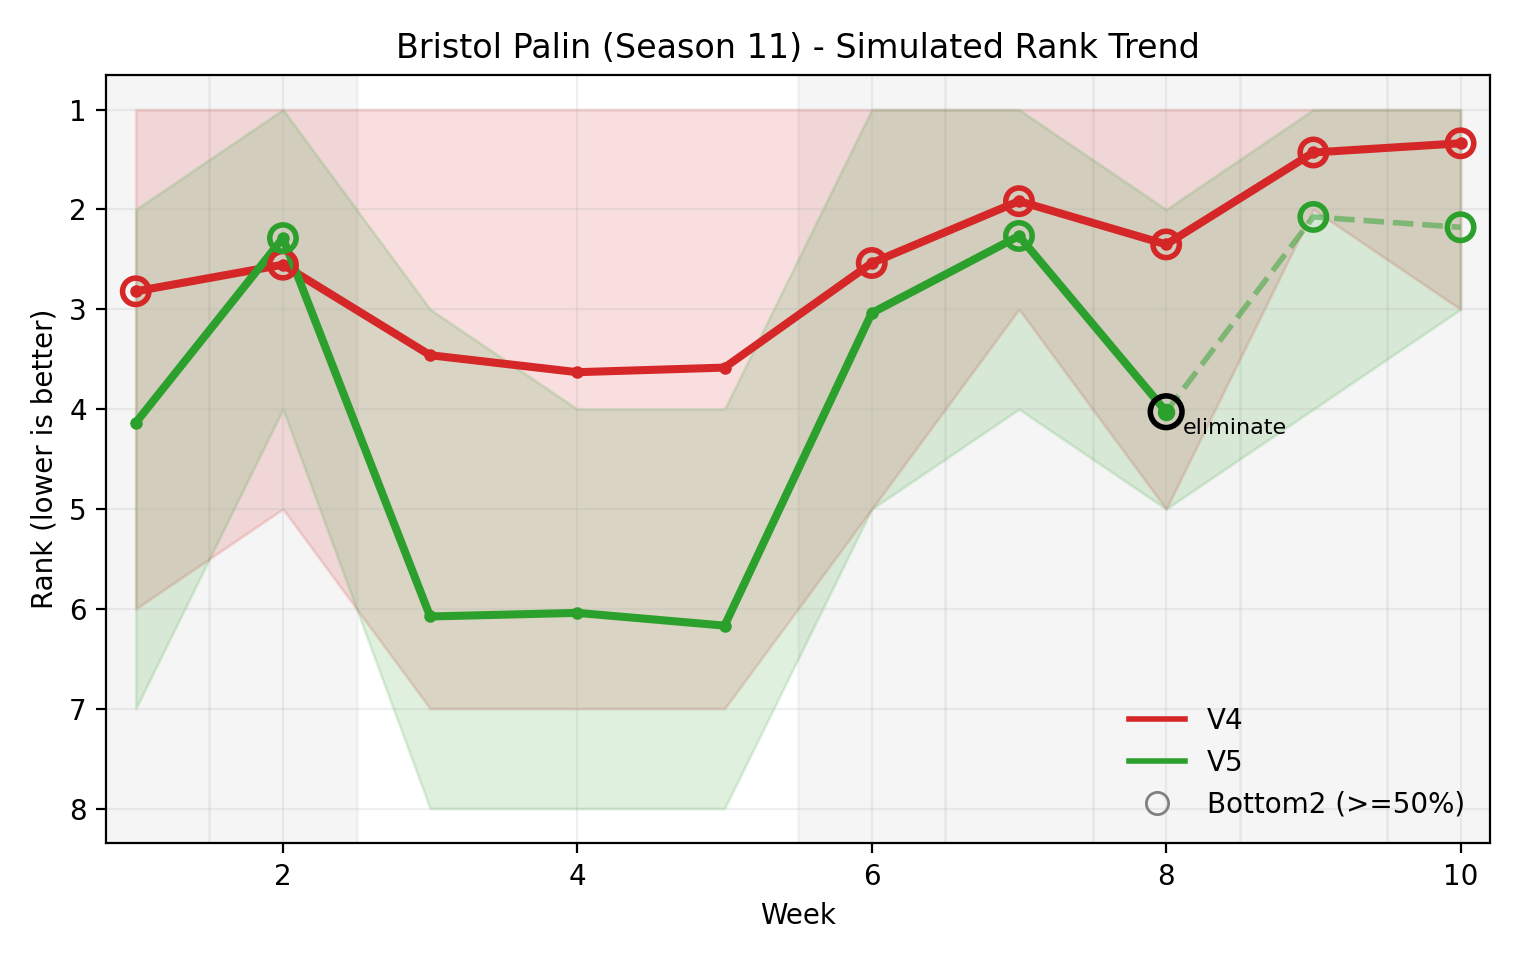
\includegraphics[width=0.32\linewidth]{8_fig_sim2_trend_11_Bristol_Palin.png} \\
			{\scriptsize Jerry Rice (S2)} &
			{\scriptsize Billy Ray Cyrus (S4)} &
			{\scriptsize Bristol Palin (S11)} \\
			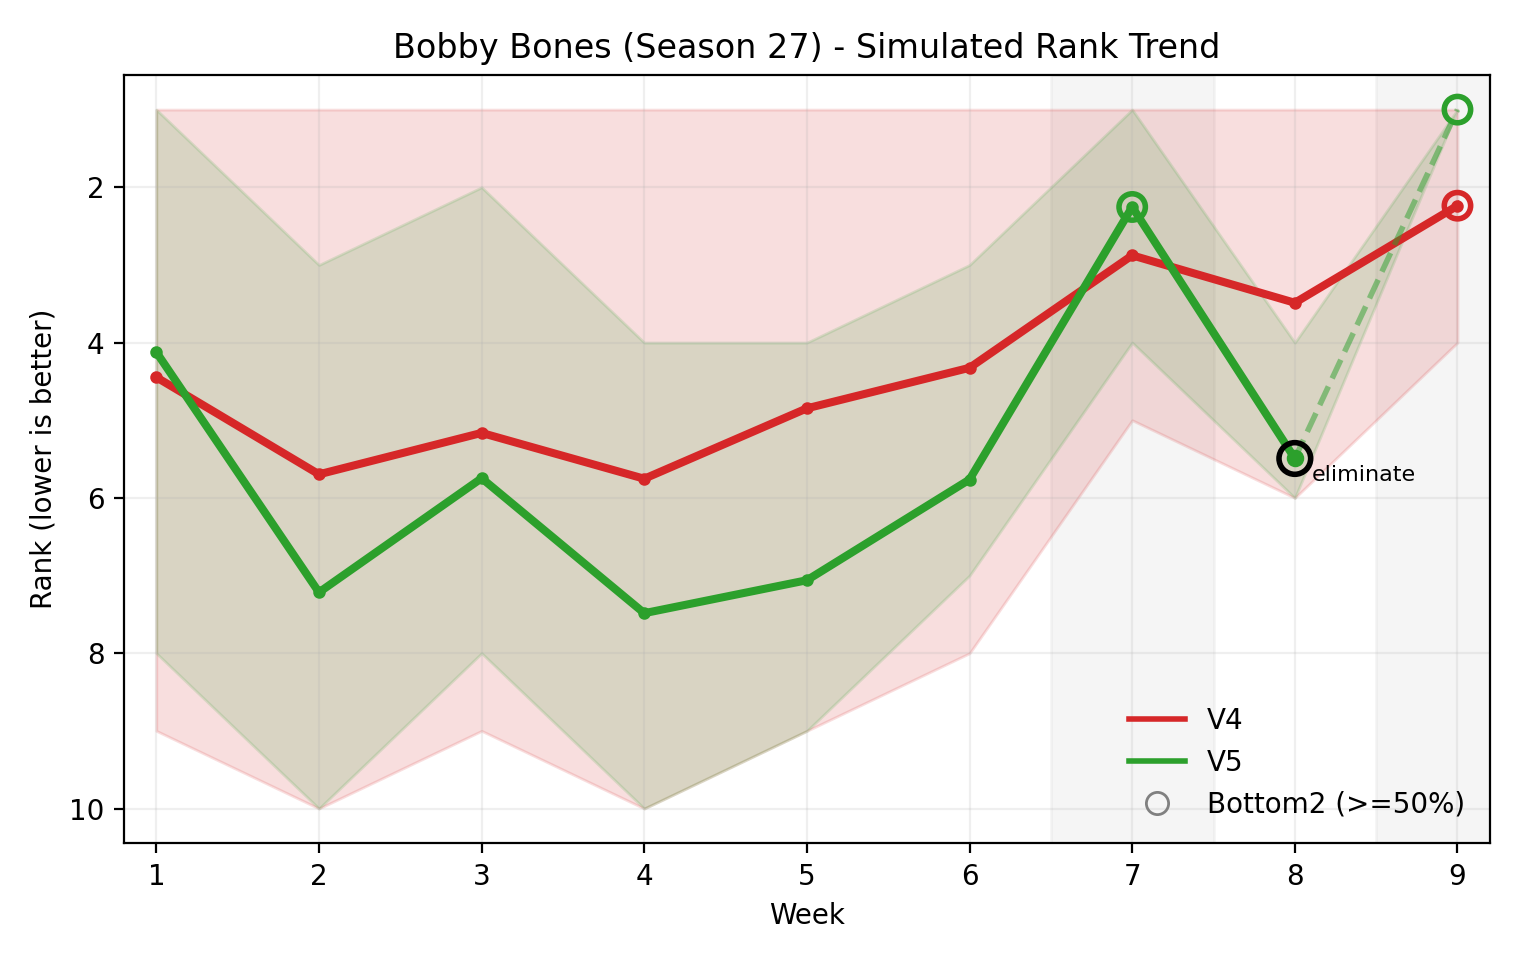
\includegraphics[width=0.32\linewidth]{8_fig_sim2_trend_27_Bobby_Bones.png} &
			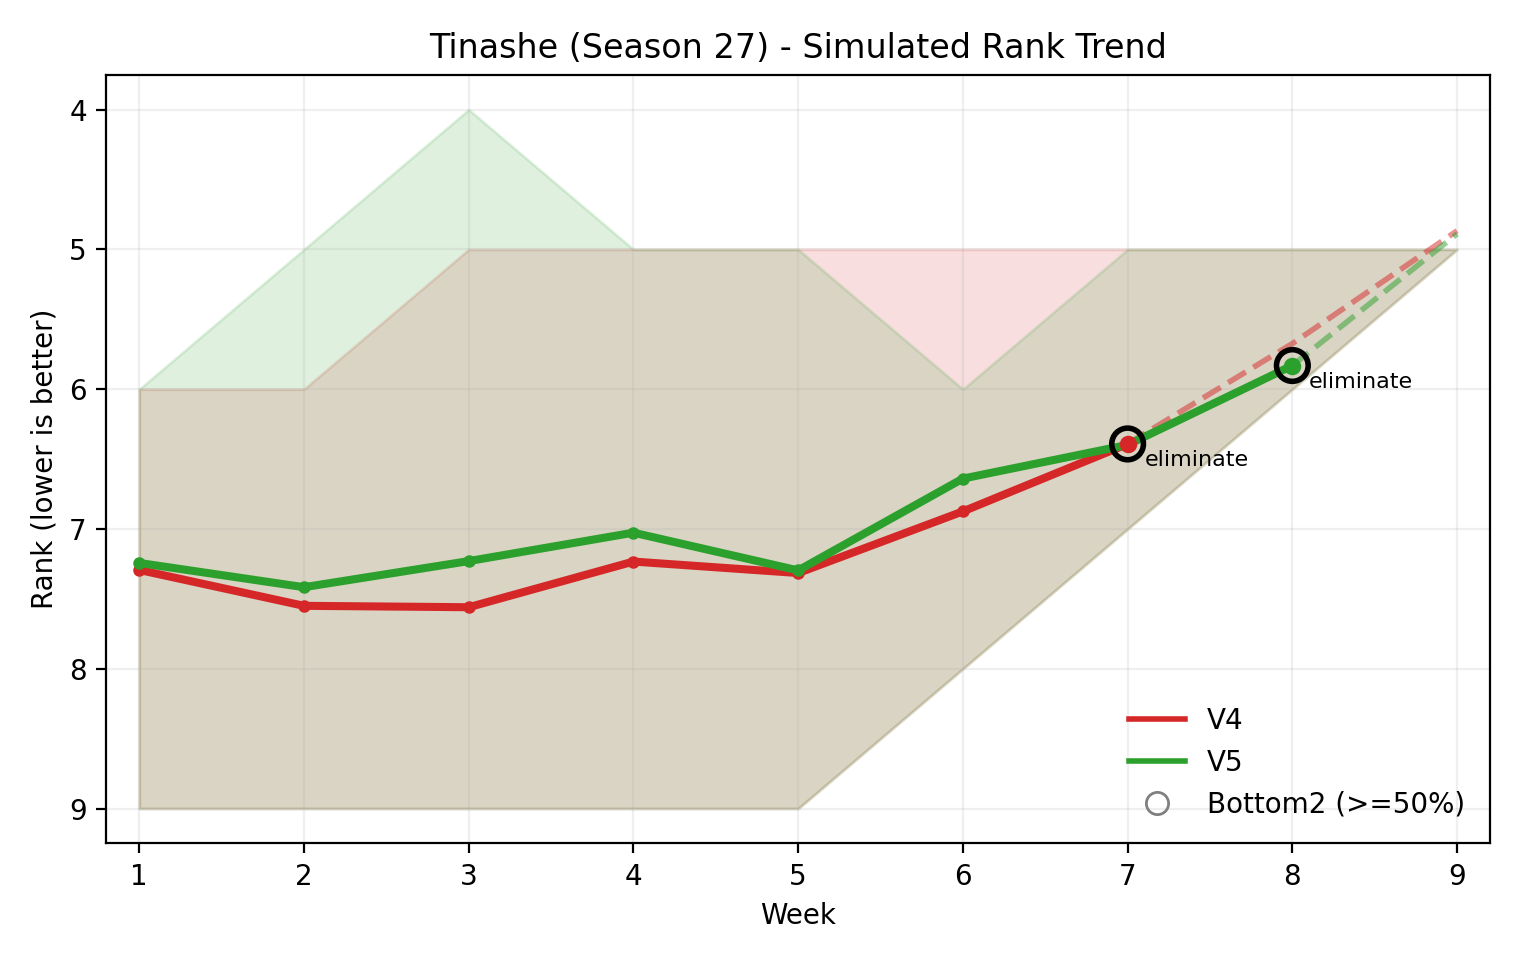
\includegraphics[width=0.32\linewidth]{8_fig_sim2_trend_27_Tinashe.png} &
			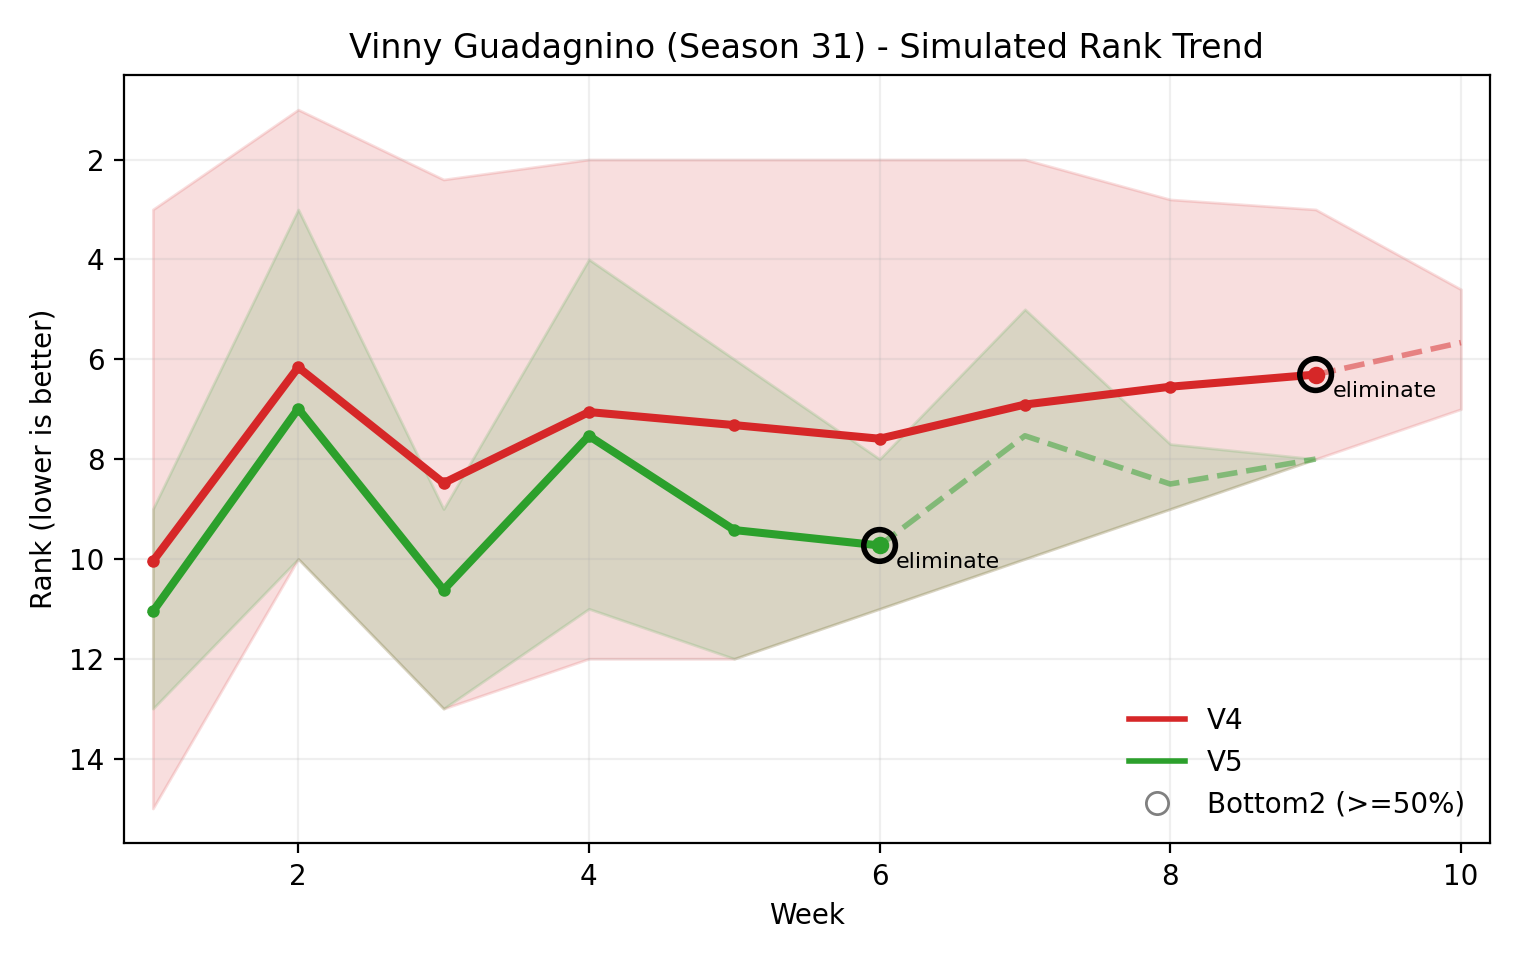
\includegraphics[width=0.32\linewidth]{8_fig_sim2_trend_31_Vinny_Guadagnino.png} \\
			{\scriptsize Bobby Bones (S27)} &
			{\scriptsize Tinashe (S27)} &
			{\scriptsize Vinny Guadagnino (S31)} \\
		\end{tabular}
		
		\vspace{0.3em}
		{\small \textbf{(b)} \textbf{Controversial cases (Baseline V0 vs V2):}
			Each mini-panel plots simulated weekly rank with posterior uncertainty bands; black rings mark high Bottom-2 incidence and ``eliminate'' marks the observed exit.}
		
	\end{minipage}
	
	\caption{\textbf{V2 reduces popularity-driven over-advancement while preserving competition dynamics.}
		(a) Unconditional survival by archetype under the baseline (V0) and V2.
		(b) Six controversial contestants: relative to baseline, V2 generally shifts trajectories toward worse ranks and/or earlier elimination risk for popularity-driven cases, with one technical-leaning case exhibiting the opposite pattern.
	}
	
	\label{fig:v2_survival_and_cases}
\end{figure}


% ---------------------------
% One paragraph: large-sample + case studies (no repetition of V1 narrative)
% ---------------------------
\paragraph{Population-Level Validation:}
Figure~\ref{fig:v2_survival_and_cases} supports three points for V2 vs.\ the baseline rank+Bottom-2 rule (V0): (i) \textbf{fairness}---tempered fan shares cap extreme popularity advantage and the judges’ save prevents severe technical injustice at exit; (ii) \textbf{excitement}---fan votes still materially determine who enters Bottom-2; (iii) \textbf{why percentage}---it enables simplex-preserving nonlinear tempering.

Under V2, the prompt’s popularity-driven controversial cases (Jerry Rice, Billy Ray Cyrus, Bristol Palin, Bobby Bones) no longer dominate; e.g., Bobby Bones drops from champion to $6$th, with similar downward corrections for the others. Meanwhile, the technical-leaning case Tinashe is protected by the judges’ save (Week~7 $\rightarrow$ Week~8).


\subsection{Policy Recommendation}
\textbf{V1 (Judge gate + fan elimination)} maximizes excitement by giving fans decisive weekly control within a judge-defined risk set, but it does not reliably curb popularity-driven over-advancement and often leaves controversial outcomes intact.

\textbf{V2 (Tempered percent + bounded merit/momentum + Bottom-2 judge save)} is fairer: tempering caps extreme fan dominance, bounded bonuses reward performance/improvement without immunity, and the judge save provides a technical safety valve while fans still shape the danger set.

\textbf{Recommendation:} choose \textbf{V2} for competitive legitimacy and \textbf{V1} for maximum engagement; a practical compromise is V1 early-season and V2 late-season (near semis/finale) for a tunable fairness--excitement balance.








\section{Sensitivity Analysis of Fan Vote Inference and Simulation}

We stress-test the fan vote inference under four perturbation families: (A1) the key hyperparameters $(\tau,\kappa)$ controlling elimination stochasticity and prior tightness, (A2) the regularization balance $\lambda_u/\lambda_\beta$, (A3) alternative judge-to-share transforms, and (A4) leave-one-season-out refits. Figure~\ref{fig:sensA_three} shows that inferred fan support is highly stable in rank order across most settings (high Spearman in the stability scatter), while PCP sensitivity is dominated by $\tau$ and secondarily by $\kappa$ (tornado). Moreover, $\text{PCP}_{\text{mean}}$ varies smoothly and monotonically with $\tau$, with larger $\kappa$ shifting PCP upward without changing the trend, indicating an interpretable and well-behaved robustness profile.

\begin{figure}[htbp]
	\centering
	
	% ---------- (a) Top: single, larger panel ----------
	\begin{minipage}[t]{0.68\textwidth}
		\centering
		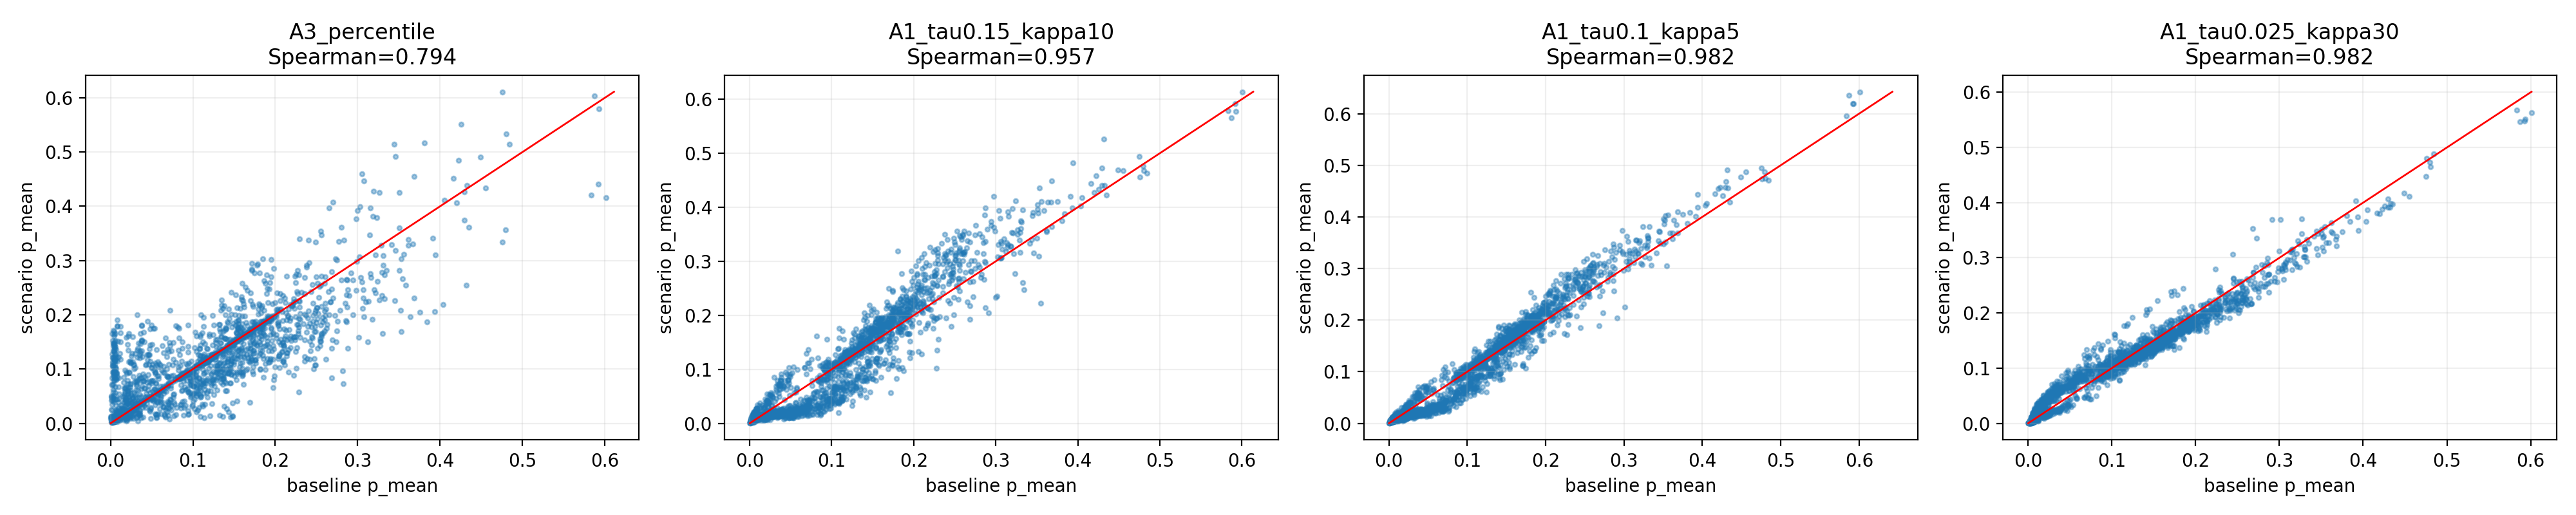
\includegraphics[width=\linewidth]{10_stability_scatter.png}
		
		\vspace{0.3em}
		{\small \textbf{(a)} \textbf{Stability of inferred fan support.}
			Baseline $p_{\text{mean}}$ versus representative sensitivity settings; high Spearman correlations indicate stable rank ordering.}
	\end{minipage}
	
	\vspace{0.6em}
	
	% ---------- (b)(c) Bottom row: closer panels ----------
	\begin{minipage}[t]{0.45\textwidth}
		\centering
		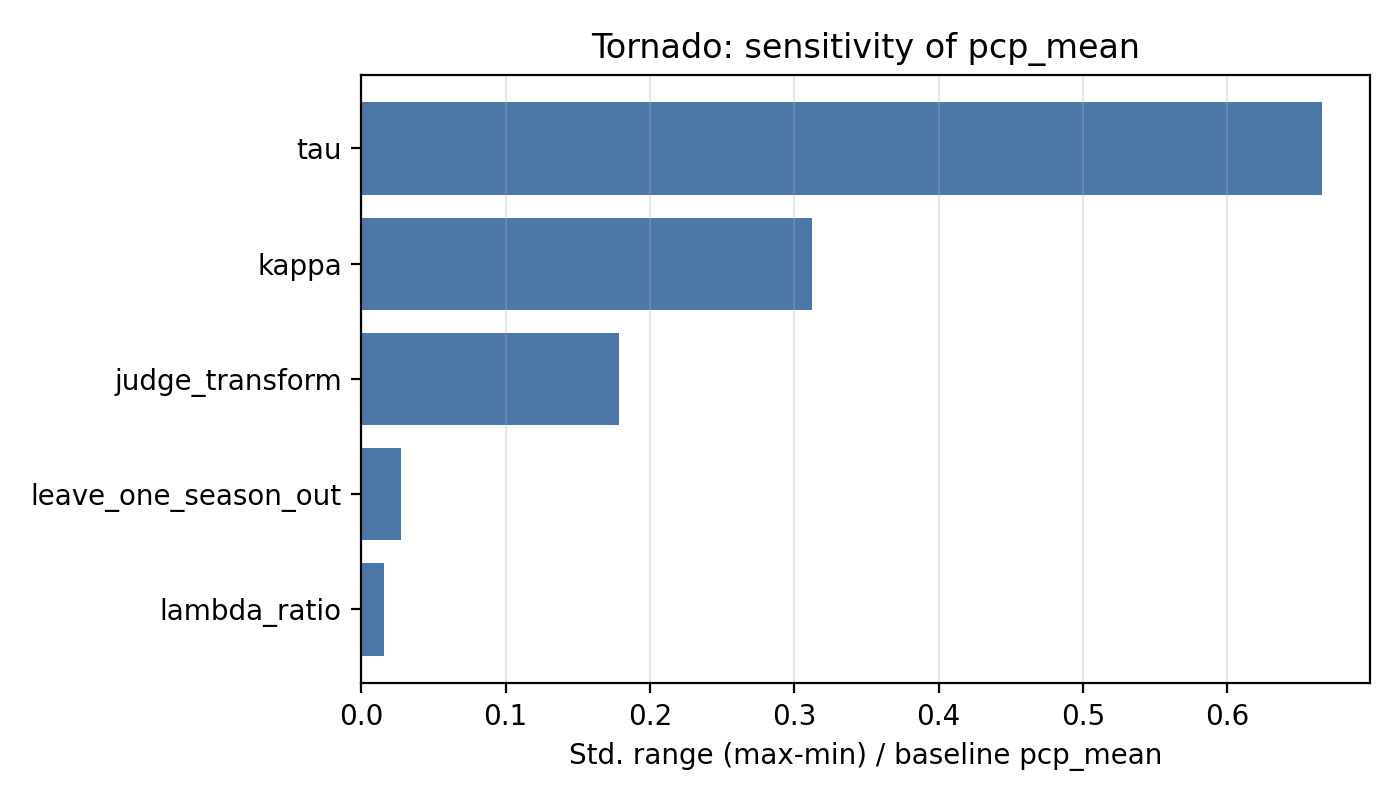
\includegraphics[width=\linewidth]{10_tornado_pcp_mean.png}
		
		\vspace{0.3em}
		{\small \textbf{(b)} \textbf{PCP sensitivity decomposition.}
			Standardized range effects show that PCP sensitivity is dominated by $\tau$, followed by $\kappa$.}
	\end{minipage}
	\hspace{0.03\textwidth}
	\begin{minipage}[t]{0.45\textwidth}
		\centering
		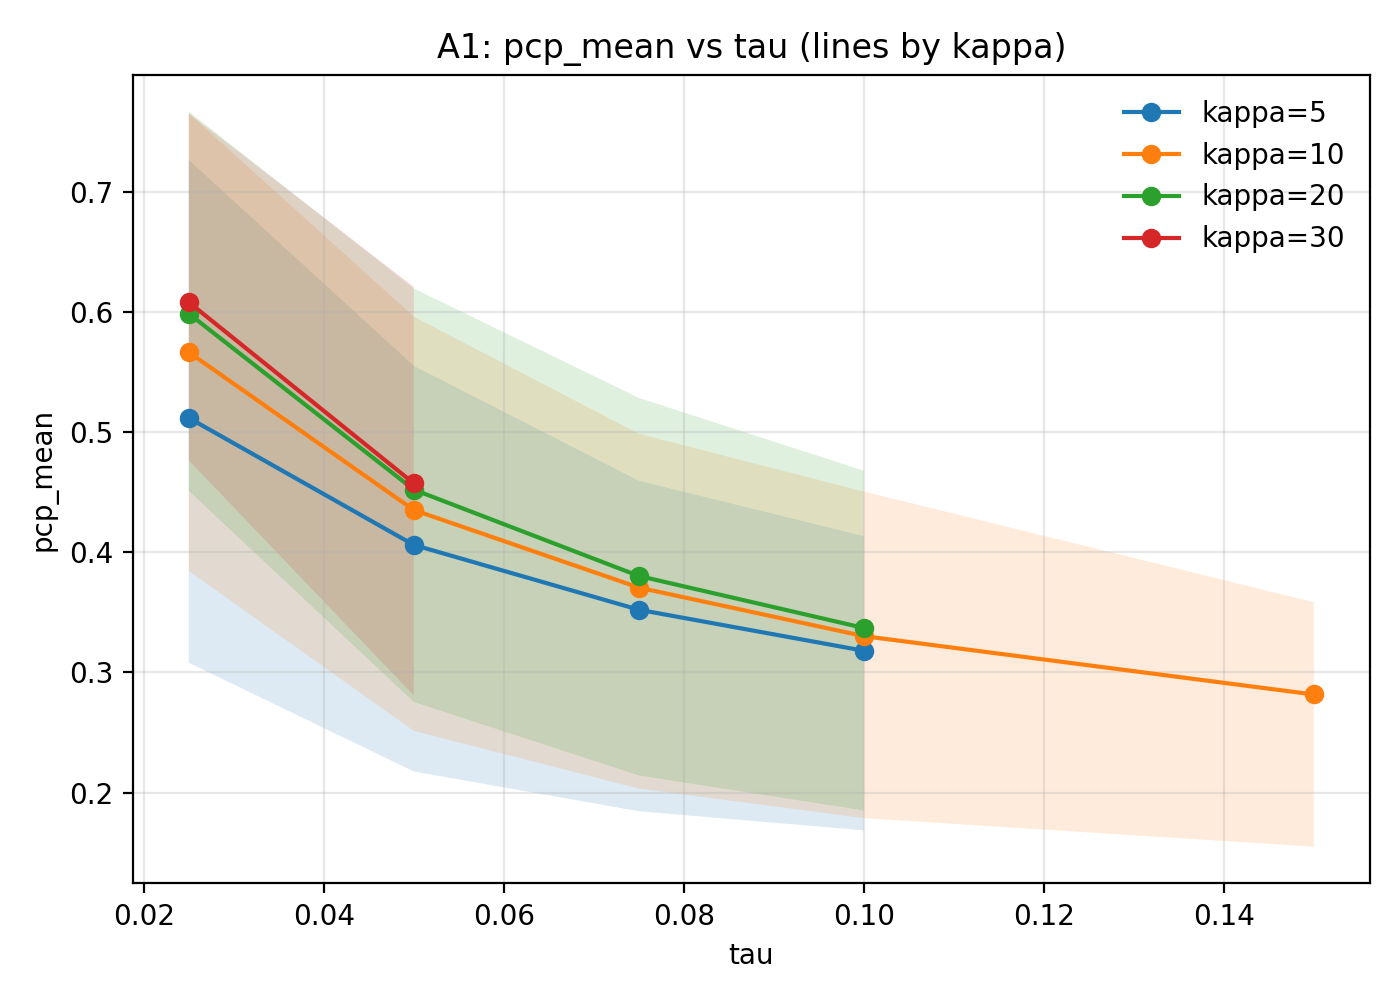
\includegraphics[width=\linewidth]{10_A1_line_pcp_mean_by_kappa.png}
		
		\vspace{0.3em}
		{\small \textbf{(c)} \textbf{Smooth dependence on $\tau$ and $\kappa$.}
			$\text{PCP}_{\text{mean}}$ decreases monotonically with $\tau$, with larger $\kappa$ uniformly shifting PCP upward.}
	\end{minipage}
	
	\caption{\textbf{Robustness of fan vote inference.}
		Inferred fan-support rankings are stable across perturbations, while PCP sensitivity is interpretable and primarily governed by the likelihood temperature $\tau$.}
	\label{fig:sensA_three}
\end{figure}

To assess the robustness of the downstream season simulator, we avoid exhaustive re-simulation and instead evaluate alternative rule variants by replaying eliminations on the same posterior fan vote draws. Across these replays, the qualitative conclusions of the simulator analysis remain unchanged, indicating that the simulation outcomes are robust to reasonable variations in rule implementation.




\section{Model Analysis}

\subsection{Strength}
\begin{itemize}
	\item \textbf{Uncertainty-aware fan-vote inference.} We combine a pooled mixed-effects popularity prior mean $q_{s,t}$, a softmin elimination likelihood on the joint judge--fan signal, and a Dirichlet posterior on the simplex (controlled by $\kappa$) updated via importance sampling, yielding posterior draws $p^{(b)}_{i,s,t}$ instead of brittle point estimates.
	\item \textbf{End-to-end, testable pipeline.} The same posterior draws drive rule replays (rank vs.\ percentage) and Monte-Carlo season simulations (V1/V2), while elimination-consistency and posterior-uncertainty summaries provide concrete diagnostics that keep conclusions reproducible and interpretable.
\end{itemize}

\subsection{Weakness and Further Discussion}
\begin{itemize}
	\item \textbf{Limited identifiability from eliminations.} Since only the eliminated couple is observed (and we exclude non-regular weeks), inference depends on correct alive sets and judge normalization; unmodeled shocks (withdrawals, special formats) may be absorbed into $p_{s,t}$, $\kappa$, or the softmin temperature $\tau$.
	\item \textbf{Mechanism attribution is confounded in V2.} Problem~4 evaluates V2 as a bundle (tempered fan shares + merit/momentum bonuses + bottom-2 judges' save), so without a full ablation we cannot isolate which component drives the fairness change; future work should run controlled ablations and separately estimate fan nonlinearity vs.\ judge-score transformations.
\end{itemize}



% ----------------------------------------------------------------
% PURE EMAIL FORMAT
% ----------------------------------------------------------------

\section*{Memorandum}

\begin{flushleft}
	\textbf{To:} \hspace{2em} Executive Producers, \textit{Strictly Come Dancing / DWTS} \\
	\textbf{From:} \hspace{0.8em} Data Strategy Team \#2623768 \\
	\textbf{Date:} \hspace{0.9em} February 2, 2026 \\
	\textbf{Re:} \hspace{2.1em} \textbf{Strategic Audit: Fixing the ``Popularity Paradox'' via Hybrid Momentum}
\end{flushleft}

\vspace{-0.5em}
\hrule
\vspace{1em}

% 设置段落间距，无需缩进
\setlength{\parindent}{0pt}
\setlength{\parskip}{1em}

We have completed a comprehensive econometric audit of over 30 seasons to identify the drivers of viewer retention and competitive integrity. Our analysis reveals a critical structural threat: the current voting mechanism allows ``Viral Anomalies'' (such as the Season 27 controversy) to hijack the competition, effectively decoupling talent from survival. To maximize franchise value, we recommend a two-pronged strategy focusing on casting efficiency and mechanism reform.

First, regarding asset allocation, our longitudinal analysis indicates that your current casting strategy is inefficient. We identified a phenomenon we call the ``Actor's Curse'': high-profile actors operate as depreciating assets, suffering from severe ``Audience Fatigue'' mid-season with a sharp drop in fan support ($\beta \approx -0.87$). Conversely, athletes and underdogs function as ``Growth Assets,'' generating significantly higher mid-season retention. We recommend shifting the casting budget towards these high-growth archetypes. If high-risk celebrities must be cast, mandatory pairing with Veteran Pros is essential; data proves veterans act as ``safety nets,'' leveraging technical scoring to extend a star's run by 2-3 weeks, thereby maximizing ad inventory.

Furthermore, the voting mechanism itself requires an overhaul to prevent ``Hostile Takeovers'' by cult fanbases. The current percentage system allows a single, massive voting bloc to render the judging panel irrelevant. Our simulations show that simple fixes like a ``Fan Save'' (V1) fail to filter these distortions. Instead, we recommend the ``Hybrid Momentum Model (V2).'' This engine applies a non-linear cap to raw fan votes to break monopolies and introduces a ``Momentum Bonus'' to reward week-over-week improvement, institutionalizing the ``Hero's Journey'' narrative. Crucially, it employs a ``Safety Valve'' where fans decide the bottom-two risk set, but judges determine the final exit, protecting premium talent from shock eliminations.

The projected impact of these changes is substantial. Running our V2 model on historical data confirms it restores brand integrity without sacrificing engagement. Under this system, the Season 27 anomaly (Bobby Bones) would have been corrected to a 6th-place finish, while technical leaders like Tinashe would have survived 30\% longer. This approach balances the viral suspense of the vote with the quality control necessary to maintain the show's long-term prestige.

\vspace{2em}

\hfill \textbf{Team \#2623768}


%References
% =========================================
% References Section
% =========================================
\addcontentsline{toc}{section}{References} % 添加到目录

\begin{thebibliography}{99}
	
	\bibitem{dwts_wiki}
	Wikipedia Contributors. (2026). \textit{Dancing with the Stars (American TV series)}. Retrieved from \url{https://en.wikipedia.org/wiki/Dancing_with_the_Stars_(American_TV_series)}
	
	\bibitem{burgoon1993}
	Burgoon, J. K. (1993). Interpersonal expectations, expectancy violations, and emotional communication. \textit{Journal of Language and Social Psychology}, 12(1-2), 30-57.
	
	% --- B. Problem 1: 核心数学模型 (混合效应/贝叶斯/Softmax) ---
	\bibitem{laird1982}
	Laird, N. M., \& Ware, J. H. (1982). Random-effects models for longitudinal data. \textit{Biometrics}, 38(4), 963-974. 
	% (支撑 Mixed-effects model)
	
	\bibitem{gelman2013}
	Gelman, A., et al. (2013). \textit{Bayesian Data Analysis} (3rd ed.). CRC Press.
	% (支撑 Bayesian posterior update)
	
	
	\bibitem{bishop2006}
	Bishop, C. M. (2006). \textit{Pattern Recognition and Machine Learning}. Springer.
	% (支撑 Dirichlet distribution & Simplex modeling)
	
	\bibitem{hoerl1970}
	Hoerl, A. E., \& Kennard, R. W. (1970). Ridge regression: Biased estimation for nonorthogonal problems. \textit{Technometrics}, 12(1), 55-67.
	% (支撑 L2 Regularization / Penalized likelihood)
	
	
	\bibitem{merton1968}
	Merton, R. K. (1968). The Matthew effect in science. \textit{Science}, 159(3810), 56-63.
	% (支撑 "Matthew Effect" / Viral Convexity)
	
	\bibitem{paharia2011}
	Paharia, N., et al. (2011). The underdog effect: The marketing of disadvantage and determination. \textit{Journal of Consumer Research}, 37(5), 775-790.
	% (支撑 "Underdog Effect" / Age penalty reversal)
	
	\bibitem{rawls1971}
	Rawls, J. (1971). \textit{A Theory of Justice}. Harvard University Press.
	
\end{thebibliography}
\clearpage

%Report on Use of AI Tools
\section*{Report on Use of AI Tools}
\addcontentsline{toc}{section}{Report on Use of AI Tools}

\begin{enumerate}
	
	\item \textbf{OpenAI ChatGPT (Jan 30, 2026 version, ChatGPT-5.2)}\\
	Query: \\
	\textit{Explain what \(\mathbf{p}_t \sim \mathrm{Dirichlet}(\boldsymbol{\alpha}_t)\) means and why it is appropriate for modeling weekly fan vote shares across remaining contestants.}\\
	Output: \\
	\textit{\(\mathbf{p}_t\) is treated as a probability vector of weekly fan vote shares that is constrained to be nonnegative and sum to one, so a Dirichlet distribution provides a natural joint model on the simplex. The parameter vector \(\boldsymbol{\alpha}_t\) controls both the expected vote shares, through \(\mathbb{E}[p_{it}] = \alpha_{it}/\sum_j \alpha_{jt}\), and the overall uncertainty via its total concentration. Different choices of \(\boldsymbol{\alpha}_t\) correspond to balanced, highly concentrated, or volatile fan support, and \(\alpha_{it}\) can be parameterized as an exponential function of judges' scores and celebrity characteristics to infer latent fan preferences when true votes are unobserved.}
	
	
	\item \textbf{OpenAI ChatGPT (Jan 30, 2026 version, ChatGPT-5.2)}\\
	Query: \\
	\textit{How is the parameter vector \(\beta\) estimated in the model \(\alpha_{it}=\exp(x_{it}^\top\beta)\), \(\mathbf{p}_t\sim\mathrm{Dirichlet}(\boldsymbol{\alpha}_t)\), when weekly fan vote shares \(\mathbf{p}_t\) are unobserved?}\\
	Output: \\
	\textit{\(\beta\) is estimated by simulated maximum likelihood using observed elimination outcomes rather than observed votes. For a candidate \(\beta\), compute \(\boldsymbol{\alpha}_t(\beta)\), repeatedly sample \(\mathbf{p}_t^{(m)}\sim\mathrm{Dirichlet}(\boldsymbol{\alpha}_t(\beta))\), apply the show’s rank/percent elimination rule with judges’ scores, and approximate \(\Pr(A_t\mid\beta)\) by the fraction of simulations that reproduce the true eliminatee \(E_t\). The season log-likelihood is then \(\ell(\beta)=\sum_t \log \Pr(A_t\mid\beta)\), and \(\hat\beta=\arg\max_\beta \ell(\beta)\) is obtained via numerical optimization (e.g., grid/random search or derivative-free methods) because the elimination rule is discrete and non-differentiable.}
	
	\item \textbf{OpenAI ChatGPT (Jan 30, 2026 version, ChatGPT-5.2)}\\
	Query: \\
	\textit{Is the final elimination or ranking determined only by the data from the elimination week or the final week, with earlier weeks used only for filtering contestants rather than accumulating scores?}\\
	Output: \\
	\textit{Yes, weekly outcomes are determined solely by that week’s judges’ scores and fan votes under the applicable rule, with no accumulation of scores across weeks. Earlier weeks affect the final result only through a survival mechanism: they determine which contestants remain eligible to enter the final week. In the finale, rankings are assigned using only final-week data among the surviving contestants, while earlier weeks influence the outcome indirectly by shaping the set of finalists rather than contributing numerically to their final ranks.}
	
	\item \textbf{OpenAI ChatGPT (Jan 30, 2026 version, ChatGPT-5.2)}\\
	Query: \\
	\textit{For Problem 1, is the ``fan vote estimation'' model simply estimating contestants' average audience voting given overall placing and judges' scores?}\\
	Output: \\
	\textit{The direction is close, but the precise target is weekly rather than season-average voting: the task is to infer a latent per-week fan vote share/strength vector that lies on the simplex and, when combined with judges' scores under the season's rule (rank- or percent-based), reproduces the observed weekly eliminations (and only in the finale week, the observed final placing). Using ``placing'' as supervision for all weeks is invalid, and describing the goal as an ``average'' fan vote model is misleading because fan support is dynamic across weeks; the correct framing is an inverse problem of recovering week-level relative vote shares consistent with the mechanism and outcomes.}
	
	\item \textbf{OpenAI ChatGPT (Jan 30, 2026 version, ChatGPT-5.2)}\\
	Query: \\
	\textit{If predicting fan rank is effectively predicting placement, and the model is trained using true placements (including weekly eliminations), does this mean the model is simply learning what it is evaluated on?}\\
	Output: \\
	\textit{This is not a circular prediction problem because the model does not directly predict placements; it infers latent fan vote ranks or shares that, when combined with known judges’ scores under fixed rules, can generate the observed outcomes. The same elimination or placement can be produced by many different fan-rank configurations, so the task is an inverse inference problem with multiple feasible solutions rather than memorizing labels. The main statistical risk is overfitting within this multi-solution space, which is addressed by imposing shared structure or regularization on fan votes and by validating consistency on held-out weeks or seasons, demonstrating that the model captures stable voting mechanisms rather than reproducing outcomes mechanically.}
	
	\item \textbf{OpenAI ChatGPT (Jan 31, 2026 version, ChatGPT-5.2)}\\
	Query: \\
	\textit{Are the bootstrap confidence intervals for the estimated parameters meaningful, and how should they be interpreted in this model?}\\
	Output: \\
	\textit{Yes, the bootstrap confidence intervals are meaningful, but they must be interpreted in light of the model structure rather than as classical regression coefficients. In this framework, \(\beta\) affects latent fan support, which in turn combines with judges’ scores to determine elimination probabilities, so the sign of \(\beta\) reflects whether a feature systematically increases or decreases inferred fan support. Bootstrap intervals are appropriate because the likelihood is highly non-linear and non-differentiable, and they capture the stability of coefficient direction and magnitude under repeated realizations of the weekly elimination process. Intervals that do not cross zero indicate robust directional effects, while wide or zero-crossing intervals reflect limited data or heterogeneous effects rather than model failure.}
	
	
	\item \textbf{OpenAI ChatGPT (Feb 1, 2026 version, ChatGPT-5.2)}\\
	Query: \\
	\textit{I plan to compare ``stay longer / reach finals'' across three contestant archetypes (technical/judge-driven, fan-driven, balanced) defined at the contestant--season level \((i,s)\) using thresholds on mean disagreement \(\overline{\Delta r}_{i,s}, \overline{\Delta s}_{i,s}\) and a persistence criterion \(\max(\pi^r_{i,s},\pi^s_{i,s})\). Are these definitions reasonable?}\\
	Output: \\
	\textit{The overall idea is sound and the unit of analysis is correctly defined as the contestant--season pair \((i,s)\), which matches season-level outcomes such as weeks survived and making the finals. The inequality directions are consistent with \(\Delta r=r^F-r^J\) (larger means judges rank the contestant higher than fans) and \(\Delta s=\hat p-J\) (negative means lower inferred fan share than judge signal), so the judge-driven and fan-driven rules align with the intended semantics. To make the persistence condition defensible, \(\pi^r,\pi^s\) should be explicitly defined as a across-week sign-consistency (or frequency) measure, and \(\tau\) as the minimum proportion of weeks required for ``sustained'' mismatch; the \(\max(\cdot)\) criterion should be justified as an OR rule across rank vs share disagreement. A practical refinement is to add a fourth ``volatile/mixed'' type (or impose low-variance constraints for the balanced type), because near-zero averages can mask frequent sign switching and would otherwise contaminate the balanced group. Thresholds \((c_r,c_s,\tau)\) should be chosen via interpretable scales or data-driven quantiles and accompanied by a simple sensitivity check showing that key group-level conclusions are stable.}
	
	\item \textbf{OpenAI ChatGPT (Feb 1, 2026 version, ChatGPT-5.2)}\\
	Query: \\
	\textit{My simulation results are the opposite of what I expected. What mechanism could actually suppress high-popularity/low-skill contestants and help high-skill/low-popularity contestants reach the finals?}\\
	Output: \\
	\textit{The reversal is plausible because in a zero-sum elimination game, constraining the worst performers does not automatically support strong-but-unpopular contestants and can even reduce uncertainty in a way that locks in early popularity advantages. Mechanisms that are more likely to work must explicitly protect or reward technical strength rather than only penalizing low performance: (i) a technical floor (hard or soft), where top-judge performers are immune or receive a strong elimination-probability discount; (ii) stage-wise objective switching, intervening in the mid-stage (e.g., 6--10 remaining) to ensure technical contestants survive before the popularity-driven endgame; and (iii) non-linear fan-weight saturation (e.g., using \(\log(p+\epsilon)\) or \(p^\gamma\) with \(\gamma<1\)) to reduce the marginal advantage of extremely high fan support. A practical combined scheme is a mid-stage technical floor plus fan-signal saturation, which directly protects high-skill/low-popularity contestants while preventing fan-dominance from overwhelming judge signals.}
	
	\item \textbf{OpenAI ChatGPT (Feb 2, 2026 version, ChatGPT-5.2)}\\
	Query: \\
	\textit{Summarize the findings from controversial contestant case studies where the proposed voting mechanism was intended to prevent technically weak but highly popular contestants from advancing, but instead failed or worsened the outcomes.}\\
	Output: \\
	\textit{The analysis showed that the revised mechanism did not resolve the historically controversial cases (e.g., Jerry Rice, Billy Ray Cyrus, Bristol Palin, Bobby Bones) and in some instances amplified the gap between low judge scores and high final placements. This indicates that the model fails to achieve its fairness objective of blocking persistently weak technical performers from advancing. The main reason is structural: bottom-$K$ nomination and elimination remain fan-dominated, effectively granting popular contestants an implicit immunity despite poor judge evaluations.}
	
	
	\item \textbf{OpenAI Codex (Feb 1, 2026 version)}\\
	Auto-completions and code suggestions were used to assist in running an existing engineering pipeline in a Jupyter Lab environment, including command-line execution of \texttt{detect.py} and \texttt{train.py}, environment setup, dependency checks, and example scripts for end-to-end data ingestion, model training, and detection using cached data and generated model snapshots.
	
	\item \textbf{OpenAI Codex (Feb 1, 2026 version)}\\
	Auto-completions and code assistance were used to design and implement visualization cells for the rank vs.\ percentage analysis, including generating week-by-week rank trajectories for selected contestants, adding uncertainty bands for posterior fan ranks, shading bottom-2 regions, and encoding probabilistic metrics (e.g., bottom-2 probability and save-elimination probability) into marker size and styling. The assistance supported integrating these figures into an existing Jupyter notebook workflow and exporting publication-ready images.
	
	\item \textbf{OpenAI Codex (Feb 1, 2026 version)}\\
	Auto-completions and code generation were used to draft a Monte Carlo season simulator (\texttt{season\_simulator.py}) that integrates the probabilistic fan-vote model (\texttt{model.py}) with contestant archetype labels (\texttt{contestant\_archetypes.csv}) and cleaned contestant data (\texttt{df\_clean.csv}). The script simulates weekly eliminations under three schemes (S1 rank+bottom2+judge save; S2 early S1 then judge-nominated \(K\) with fan elimination; S3 full judge-nominated \(K\) with fan elimination, with finals ranked by combined scores), supports an early/late split by cumulative eliminations (\(m\)), and outputs per-simulation detail and scheme/archetype weekly summaries (advancement, average rank, elimination rates) for comparing impacts on fan-driven, judge-driven, and balanced contestants.
	
	
\end{enumerate}

\end{document} 